\documentclass[journal]{IEEEtran}
\usepackage{amsmath,amssymb,graphicx,booktabs,array,cite,url}
\renewcommand{\ttdefault}{cmtt}
\usepackage[hidelinks]{hyperref}
\hypersetup{pdftitle={Supplement: Structured Channel Estimation for Rydberg Arrays With Learned Filtering and Observable Recovery Checks},pdfauthor={Abdullah Haatim}}
\graphicspath{{figures/}{support/figures/}}
\makeatletter
\def\input@path{{support/}}
\makeatother
\newcommand{\Hank}{\mathcal H}
\newcommand{\CN}{\mathcal{CN}}
\newcommand{\R}{\mathbb R}
\DeclareMathOperator{\diag}{diag}
\DeclareMathOperator{\rank}{rank}
\DeclareMathOperator{\tr}{tr}
\begin{document}
\title{Supplement to: Structured Channel Estimation for Rydberg Arrays With Learned Filtering and Observable Recovery Checks}
\author{Abdullah~Haatim}
\maketitle
\begin{abstract}
This supplement specifies the final receiver's policy, algebraic validity conditions, development/confirmation protocol, adverse cases and numerical evidence. It then preserves the classical and learned studies from which the receiver developed. Historical experiments retain their own models, data, metrics and inference procedures; statements about a historical primary method or final bank refer only to that study. The new receiver is the matched-context hybrid with the confirmed residual-triggered algebraic fallback. No historical table is pooled with its fresh 153-condition comparison. The supplementary evidence is a summary and provenance archive, not a full public raw-data and checkpoint release.
\end{abstract}

\section{Final Receiver: Stored Components and Exact Policy}
The current receiver uses the matched-30-context adaptive and global fits for seeds 9101, 9102 and 9103. One paired inference fit stores 218 neural parameters; reported fit means average metrics and do not ensemble channels. Its observation inputs are $Z,S,B,v$, with $N=32$, $K=3$, $P=30$ in the final experiment. The complete policy and checkpoint/source hashes are supplied in \texttt{evidence/reliability/source/policy.json} and the protocol record. True channel, path count and test error are not routing inputs.

Let $s=10\log_{10}(K/v)$ and $r=10\log_{10}\operatorname{mean}|B|^2$. Reference keys are nearest to 5, 12 and 20~dB; SNR keys are nearest to the declared 17-point grid. Exact ties select the lower key. A tolerance of $10^{-10}$~dB is used at the continuous boundaries. The adaptive start is used for $s\le30+10^{-10}$, the global schedule above it. At $s\le20+10^{-10}$, return the raw adaptive output exactly. Elsewhere use Table~\ref{tab:final-policy}. If the family's lookup record disagrees with continuous model routing, extra EM is set to zero. It is a deterministic off-grid rule, not interpolation or a guarantee of smooth performance.

\begin{table*}[!t]
\centering\small
\caption{Frozen prior-hybrid table inherited by the final receiver. Entries are extra EM updates and final noise-scale multiplier $c$. Ref denotes nearest-reference key. EM starts from the chosen trained output. At SNR at most 20~dB both continuation and final filtering are bypassed.}
\label{tab:final-policy}
\begin{tabular}{@{}lrrrrrr@{}}\toprule
SNR key (dB)&$T$, ref 5&$T$, ref 12&$T$, ref 20&$c$, ref 5&$c$, ref 12&$c$, ref 20\\\midrule
0--30&0&0&0&0&0&0\\
32.5&0&10&10&0&2&2\\
35&0&10&40&0&2&4\\
37.5&0&20&40&0&4&4\\
40, 42.5, 45&40&20&40&0&4&4\\
50, 60&40&40&40&0&4&4\\\bottomrule
\end{tabular}
\end{table*}

The final filter applies the same smooth Hankel map as the trained stages with $\beta=1$ and
\begin{equation}
 \tau_k=c\sqrt{2v\operatorname{Re}[(SS^H)^{-1}]_{kk}\max(m,q)}.
\end{equation}
For $c=0$, it returns its input exactly. Positive $c$ gives a decreasing threshold as supplied noise decreases; it is a heuristic scale, not a theorem about the noise covariance after EM. Maintaining this filter above 40~dB removed an earlier artificial switch-off, while other piecewise transitions remain.

Only cases in the nearest-reference 5~dB bin with $s>30+10^{-10}$ enter the new diagnostic. The complete incumbent $G_0$ is computed first. The maximum antenna residual
\begin{equation}
 \max_n\frac{2}{Pv}\sum_p[Z_{np}-|[G_0S+B]_{np}|]^2
\end{equation}
exceeding 2 triggers one algebraic start, 20 exact EM updates and the same final-filter rule. The complete fallback replaces the incumbent only if finite and its average fitting Rician negative log-likelihood is smaller by more than $10^{-12}$. Failed solves, no triggers and rejected alternatives return the incumbent bitwise. The standalone algebraic-start-plus-EM20 baseline instead applies the algebraic start on every condition and uses spectral-plus-EM20 when that solve is invalid.

\section{Intensity Regression: Coefficients, Noise and Scope}
For repeated $b_n\ne0$, define $c_n=g_n/b_n$ and $y_{np}=(Z_{np}^2-v)/|b_n|^2-1$. The expansion is
\begin{align}
 \mathbb E[y_{np}]={}&2\operatorname{Re}\sum_i c_{ni}s_{ip}
 +\sum_i|c_{ni}|^2|s_{ip}|^2\nonumber\\
 &+2\operatorname{Re}\sum_{i<j}c_{ni}c_{nj}^*s_{ip}s_{jp}^*.
\end{align}
All expectations here condition on $G,S,B$. The corresponding real coefficients are the real/imaginary components of $c_n$, its three squared magnitudes and the real/imaginary components of each pair product. The signs of the imaginary columns are negative because $\operatorname{Re}(ab)=\operatorname{Re}a\operatorname{Re}b-\operatorname{Im}a\operatorname{Im}b$. There are $d=2K+K^2=15$ columns for three users. The real least-squares solution treats the quadratic coefficients as nuisance variables; it does not enforce their consistency with a rank-one outer product.

Writing $y_n=D\xi_n+\epsilon_n$ gives $\mathbb E\epsilon_n=0$ and
\begin{equation}
 \operatorname{var}(\epsilon_{np})=
 \frac{2v|g_n^Ts_p+b_n|^2+v^2}{|b_n|^4}.
\end{equation}
Independent field noise makes this conditional covariance diagonal over pilots. If $D$ has full column rank, $\widehat\xi_n=(D^TD)^{-1}D^Ty_n$ is conditionally unbiased and has covariance
\begin{equation}
 (D^TD)^{-1}D^T\operatorname{cov}(\epsilon_n)D(D^TD)^{-1}.
\end{equation}
These formulas explain sensitivity to conditioning and noise/reference scale. The ordinary least-squares solve is not asserted to be minimum variance. At $v=0$, $\epsilon_n=0$ and full rank recovers $c_n$ exactly. In floating-point tests, the independent noiseless algebraic reconstruction errors were of order $10^{-15}$.

The implementation uses SVD least squares, checks rank 15 and condition number at most $10^8$, and rejects nonfinite coefficients or a reference that does not repeat exactly. With constant-modulus pilots, each diagonal design column is a constant vector, so three such columns span at most one dimension and rank is at most 13. The current validity rule then rejects. A reduced parameterization could remove this redundancy, but is not implemented or tested here. Extra offline known QPSK probes and online QPSK data must not be confused with the Gaussian fitting pilots. Neither unbiasedness of the unselected initializer nor noiseless exactness extends automatically to the refined, filtered, selected receiver.

\section{Training, Offline Selection and Independent Confirmation}
The final adaptive and global models train on the same 39-observation blocks, using 30 fitting observations and 9 held out. Training/validation block counts are 16,384/2,048, batch size 32, epochs 20 and Adam learning rate 0.001. The validation score equally averages 126 SNR/reference/path strata. All three fit seeds share this data population; model fits and data-population replications are different uncertainties. The older 21-context and re-corruption experiments retained later in this supplement are separate recipes.

Each new policy bank A/C has 768 independent physical anchors (256 in each of three path regimes), reference 5~dB and eight coupled SNRs above 30~dB. It supplies 30 context observations, 9 independent held-out Gaussian observations and 64 known-symbol probes per channel. Ground-truth channels are used by the simulator but are not exported to development selection. The 12 rules cross two residual summaries, thresholds 2/4/8 and tails 10/20. All pass the separate complete-pipeline calibration cap of 10~ms p90; 144 forced-fallback calls separately exercise longer branches.

Selection requires positive held-out-loss gain and empirical probe-error nonincrease in every path regime. The incumbent is always admissible, and tie rules are fixed. The chosen maximum/2/20 rule triggers on 27.848\% of A cases and 27.837\% of C cases, averaging fits. C's one-sided 95\% lower loss-gain bound is 0.198729; its descriptive two-sided 95\% interval is [0.195729, 0.370585]. Both methods have zero observed probe errors in each regime. Only the selected rule is confirmed; no substitute is searched on C or the final test. This confirms the incremental wrapper under the protocol, not every earlier inherited EM-tail decision.

The current fresh test uses 1,152 independent anchors in nine reference/path blocks and 19,584 coupled SNR condition cases. Data BER uses 7,520,256 bits per fit. The bootstrap shares within-block indices over SNR, methods and fits and draws independently across blocks. The four whole-grid outcome intervals are multiplicity adjusted; regional and per-cell intervals remain descriptive. The evidence archive preserves all raw counts and per-fit summaries available in the compact source records.

\section{Exact Baseline Definitions and Frozen Selection}
\label{sec:baseline-reproduction}
The directory \path{evidence/reliability/baselines/} contains byte-for-byte copies of the inherited baseline policies and their selection records. \path{PROVENANCE.json} gives each original repository path, SHA-256 digest and copy size, plus the implementation-source hashes. \path{policy_summary.json} expands all 51 reference/SNR entries into the compact configuration and the full-repair base/filter combination. This is a reporting transformation of frozen records, not a new selection. Baseline parameters were not reoptimized on the final reliability development or test banks.

\subsection{Classical Structured Start and Common-40 Controls}
The classical start uses the same spectral initializer as the learned starts, followed by ten exact EM updates with unit relaxation. Each update is followed by smooth Hankel filtering and mixing. Its single global configuration was selected from 30 choices: relative thresholds $\{0.01,0.03,0.1,0.3,1\}$ or noise multipliers $\{0.5,1,2,4,8\}$, each crossed with mixing $\{0.1,0.5,1\}$. Relative thresholds multiply the current Hankel RMS; noise thresholds use the formula in the final-filter section. The criterion is the minimum raw-start held-out Rician loss, averaged equally over the 126 strata of the same 2,048 validation blocks and fixed 30/9 split used for the learned checkpoint selection. No extra EM continuation or post-start final filter enters this selection score. Evaluation uses double precision on the stored single-precision observations.

The selected start has noise multiplier $c=1$ and mixing $\beta=1$ at every stage. The complete classical-start-plus-EM40 control then adds 40 unfiltered exact EM updates and the final-filter table in Table~\ref{tab:final-policy}. The adaptive-start-plus-EM40 and global-schedule-plus-EM40 controls use the corresponding trained start with these same 40 updates and final filter, including at ordinary SNR; they do not use the hybrid's ordinary-SNR bypass. \path{classical_selection.json} retains all 30 candidate scores and their 126 stratum scores. The copied start-ablation protocol records this selection; the start-budget protocol/policy records the subsequent common-40 comparison. Selection on raw-start likelihood does not guarantee an optimal configuration for the final refined pipeline or for NMSE.

\subsection{Compact Sparse/EM Control}
Let $A_D$ have entries $[A_D]_{nj}=N^{-1/2}\exp[-\mathrm{i}n(-\pi+2\pi j/D)]$, with $n=0,\ldots,N-1$ and $j=0,\ldots,D-1$, and write $G=A_DX$. The penalized control uses a finite-iteration solver for
\begin{equation}
 \begin{gathered}
 \frac{v}{2}\sum_{n,p}\ell(Z_{np},[A_DXS+B]_{np},v)
 +\lambda\sum_{j,k}|X_{jk}|,\\
 \lambda=f\sqrt{vP\log D}.
 \end{gathered}
\end{equation}
It initializes $G$ spectrally and $X=(N/D)A_D^HG$, computes the exact Rician posterior field at each outer step, and performs the declared number of monotone-restarted FISTA inner updates on the penalized quadratic surrogate. The step size is $[(D/N)\lambda_{\max}(SS^H)]^{-1}$. Coefficients carry between outer steps; finite inner iteration counts are not exact penalized M-step solves. FFT products implement this uniformly spaced spatial-frequency dictionary. The zero-penalty option directly performs 100 unregularized EM updates and does not run a redundant sparse solve.

The compact menu contains three $(D,\hbox{inner},\hbox{outer})$ structures, $(128,8,12)$, $(256,8,12)$ and $(256,2,40)$, each with $f\in\{0.03,0.1,0.3,1,3\}$, plus direct EM100. At the last sparse refresh, all 16 passed the historical complete-pipeline calibration cap of 10.7439662~ms, defined by the contemporaneous full-repair pooled p90. Only the ten bins at references 12/20~dB and SNR 40/42.5/45/50/60~dB were refreshed: 384 development anchors per path regime supplied 30 fitting and nine independently drawn held-out pilots. Minimum equally weighted held-out Rician loss selected the configuration; exact score ties used calibration p90 then candidate name. The other 41 bins retained the preceding frozen policy. These historical eligibility times are not substituted for the final experiment's fresh latency measurements, and this compact menu is not a globally optimized classical accuracy--time frontier.

\path{filter_continuation_policy.json} includes every compact configuration and the last refresh's candidate scores; its copied protocol and calibration preserve the menu, bank hashes and timing evidence. The final table has 34 penalized entries and 17 direct-EM100 entries. Nearest-reference/SNR lookup chooses the lower bin at a tie; there is no online rank search or validation split. All 30 deployment pilots are used to estimate the channel.

\subsection{Earlier Full Repaired Receiver}
The full-repair comparator uses the matched-context adaptive start, not the global schedule. At reference 5~dB it returns that start through SNR 32.5~dB, adds five exact EM updates at 35~dB, and adds 100 from 37.5~dB upward. At reference 12~dB it returns the adaptive start through 30~dB; at 32.5/35~dB it adds 2/5 EM updates and final filtering with $c=2$; from 37.5~dB upward it uses spectral EM100 followed by $c=4$ filtering. At reference 20~dB it returns the adaptive start through 30~dB, adds 3 EM updates and $c=2$ filtering at 32.5~dB, and uses spectral EM100 with $c=4$ from 35~dB upward. Final mixing is one, and all thresholds use the supplied variance. These are grid-key descriptions; off-grid inputs use the same nearest-bin rule. The copied filter-continuation policy stores the outer repair choices, while \path{dual_guard_policy.json} identifies the base beneath each final shrink operation. The native-runtime policy/protocol verifies that numerical optimization preserved these choices and the compact table. Neither baseline acquires the final receiver's algebraic recovery check.

\section{Final Effects, Adverse Conditions and Timing}
\begin{table*}[!t]
\centering
\caption{Paired whole-grid improvements relative to each reference. Positive values favor the reliability receiver.}
\label{tab:reliability-effects}
\small
\setlength{\tabcolsep}{4pt}
\begin{tabular}{llrrrr}
\toprule
Reference & Interval & \shortstack{NMSE gain\\(dB)} & Interval (dB) & \shortstack{BER reduction\\(pp)} & Interval (pp) \\
\midrule
Prior selective EM & Adjusted & 0.507 & [0.338, 0.652] & 0.000000 & [0.000000, 0.000000] \\
Full repair & Adjusted & 0.762 & [0.231, 0.878] & 0.000075 & [0.000000, 0.000266] \\
Compact sparse/EM & Pointwise & 6.725 & [5.982, 7.103] & -0.033337 & [-0.038164, -0.028612] \\
Adaptive + EM40 & Pointwise & 2.929 & [2.530, 2.994] & 0.285708 & [0.276258, 0.295150] \\
Global + EM40 & Pointwise & 2.138 & [2.076, 2.203] & 0.291222 & [0.281662, 0.300876] \\
Classical + EM40 & Pointwise & 6.615 & [5.659, 7.023] & 0.286892 & [0.277353, 0.296422] \\
Spectral EM100 & Pointwise & 8.058 & [6.900, 8.500] & 0.306333 & [0.296501, 0.316262] \\
Algebraic + EM20 & Pointwise & 2.087 & [2.002, 2.179] & 0.313181 & [0.303354, 0.323074] \\
\bottomrule
\end{tabular}
\par\vspace{2pt}
\begin{minipage}{0.98\textwidth}\footnotesize Adjusted rows use 98.75\% percentile intervals (Bonferroni across two contrasts and two outcomes for nominal 95\% family coverage). Other rows use descriptive 95\% intervals. The 20,000 resamples are paired within nine independent reference/path blocks; channel indices are shared across SNRs and fits within a block. Inference is conditional on the fixed fits, policy, and simulation grid. A collapsed empirical BER interval does not establish equivalence or noninferiority.\end{minipage}
\end{table*}
\begin{table*}[!t]
\centering
\caption{Condition-level adverse results out of 153 conditions.}
\label{tab:reliability-harms}
\small
\setlength{\tabcolsep}{4pt}
\begin{tabular}{lrrrrr}
\toprule
Reference & \shortstack{NMSE\\worse} & \shortstack{NMSE\\harm CI} & \shortstack{BER\\worse} & \shortstack{BER\\harm CI} & \shortstack{Worst NMSE\\gain (dB)} \\
\midrule
Prior selective EM & 0 & 0 & 0 & 0 & 0.000 \\
Full repair & 32 & 8 & 0 & 0 & -0.701 \\
Compact sparse/EM & 22 & 20 & 22 & 12 & -1.214 \\
Adaptive + EM40 & 29 & 12 & 3 & 0 & -3.747 \\
Global + EM40 & 20 & 10 & 3 & 0 & -3.736 \\
Classical + EM40 & 24 & 2 & 3 & 0 & -0.700 \\
Spectral EM100 & 3 & 2 & 3 & 0 & -0.701 \\
Algebraic + EM20 & 44 & 15 & 3 & 0 & -3.746 \\
\bottomrule
\end{tabular}
\par\vspace{2pt}
\begin{minipage}{0.98\textwidth}\footnotesize Worse means a negative point improvement; harm CI means a descriptive pointwise 95\% interval lies below zero. Complete adverse condition identifiers, fit effects, and intervals are retained in the archived summaries. No multiplicity-adjusted subgroup safety claim is made.\end{minipage}
\end{table*}
\begin{table*}[!t]
\centering
\caption{Individual receiver timing extremes, retaining both windows.}
\label{tab:reliability-latency}
\small
\setlength{\tabcolsep}{4pt}
\begin{tabular}{lrrllrrl}
\toprule
Window & Maximum (ms) & $>10.74$ ms & Fit & Paths & RSR/SNR (dB) & Index & Gate \\
\midrule
Window 1 & 5.225209 & 0/1377 & 9102 & Random 3--7 & 5/50 & 500 & false \\
Window 2 & 22.275833 & 1/1377 & 9103 & Random 3--7 & 12/45 & 600 & false \\
\bottomrule
\end{tabular}
\par\vspace{2pt}
\begin{minipage}{0.98\textwidth}\footnotesize The second window contains one 22.275833~ms call despite satisfying both p90 targets. Its gate was false; these measurements do not establish the cause. Pooled p90 eligibility is not a hard per-call deadline.\end{minipage}
\end{table*}

The final primary and regional tables are in the main manuscript. Here the extended effects retain fit dependence and adverse comparisons. No condition-mean NMSE or BER worsens against the prior hybrid in this bank. Against the full repair, 32 NMSE means are worse, with 8 pointwise intervals excluding zero; these are not simultaneous discoveries after correction over 153 cells. The worst loss, 0.700957~dB, is at two paths, reference 20~dB, SNR 32.5~dB, outside the new gate. Compact sparse/EM remains better for aggregate BER and pooled linear NMSE. Zero target-region bit errors do not prove equivalence or exclude rare failures.

Each timing window contains 27 independent physical anchors reused across SNR, giving 459 condition cases and 8,721 calls. Every raw/family quantile, ordering and pass flag was independently checked. The second window is slower for the baselines as well as the receiver. All three receiver fits pass the full-grid and target p90 requirements in both windows, and none of the 51 reference/SNR-bin p90 values exceeds 10.74~ms. Individual timing is different: one of 1,377 receiver calls in window 2 took 22.275833~ms. It was fit 9103, random 3--7 paths, reference 12~dB, SNR 45~dB, anchor index 600, with its gate false. The measurement does not establish a cause. No timing window was rerun to pass.

\section{Development Sequence and Interpretation}
The following sequence records what motivated the final design. Scores from its different banks are not a common leaderboard. Detailed report paths and hashes are in \texttt{historical\_report\_index.json} inside the evidence folder.
\begin{enumerate}
\item \emph{Runtime-matched sparse comparison.} An angle-domain Rician-likelihood baseline was adapted and selected under a processing budget, strengthening the classical comparator. Its final frozen form includes a direct-EM option.
\item \emph{Pilot-matched retraining and short EM.} Comparing 30 versus 21 context pilots on paired 39-observation blocks gives 0.219~dB NMSE gain and 0.01758 percentage-point BER reduction on that separate test, with adjusted intervals [0.205, 0.233]~dB and [0.01303, 0.02245] percentage points. All selected ordinary-SNR extra tails are zero; fixed 1/2/5-step continuations harm the tested adaptive estimate. The study supports matching training inputs, not a generic claim that more EM helps.
\item \emph{Retrained high-SNR bypass.} A broad high-SNR gain still leaves eight adverse conditions, with worst loss 16.415~dB. A single coarse bypass is insufficient near weak-reference transitions.
\item \emph{Weak-reference transition and incumbent-preserving repairs.} Subsequent transition, incumbent and dual-guard studies reduce specific failures but reveal regressions against earlier versions. They are development evidence for candidate generation and acceptance logic, not proof of a uniformly better filter. The first transition repair improves its weak 18-condition region by 16.208~dB but still has 10 whole-grid NMSE losses and misses its target-region p90 cap at 11.258~ms.
\item \emph{Filter continuation above 40~dB.} Keeping the strong-reference noise-scaled filter active changes 30 strong/high conditions while preserving 123 others. Its separate mean shifts from $-53.364$ to $-58.557$~dB with zero observed target BER in both. This diagnoses an artificial filter-removal jump.
\item \emph{Native runtime repair.} Numerical-kernel optimization preserves the same formulas, with recorded coefficient discrepancy at most $6.66\times10^{-14}$ in its parity checks. It is an implementation improvement, not a new estimator-accuracy result.
\item \emph{Matched starts and common continuation.} Adaptive, global and classical structured starts were compared with common EM/filtering. In the common 40-tail comparison, adaptive starts lose 0.696~dB to the global schedule on mean NMSE, while improving BER by 0.005984 percentage points. Forced 40-step refinement loses 4.808~dB in ordinary-SNR adaptive performance. This motivates preserving the ordinary branch and using different high-SNR effort.
\item \emph{Hybrid routing and selective tails.} The zero-tail hybrid underperforms the full repair. It was retained after independent confirmation rejected all proposed nonzero tails. Exploratory nonzero-tail proposals improve that hybrid, but all 21 earlier C confirmation decisions reject the proposed changes. The final reliability experiment explicitly adopts that frozen exploratory prior as its incumbent; its new confirmation does not erase these failures.
\item \emph{Current reliability wrapper.} A new, independently calibrated residual gate and different initializer are confirmed before the fresh final test. Only this current experiment supplies the main manuscript's final nine-method comparison and timing verdict.
\end{enumerate}

\section{Evidence Integrity and Reproduction Scope}
The source bundle includes compact final protocols, policy, source/checkpoint hashes, all-method summaries, adverse-cell lists, timing records, five audits, figure values and 163 independently checked numerical table entries. It excludes the large raw NPZ banks and neural checkpoint binaries. Compilation requires only the included figures, bibliography and TeX sources. Regenerating simulations requires the original code/data environment or a future complete public release; no archive DOI has been invented.

The final selection audit reconstructed development observations and decisions before test generation. Independent base and fallback prediction replays match exactly. The test audit replays 2,448 standalone predictions, independently rebuilds 9,216 gate/fit cases and verifies ordinary output preservation. The BER audit independently checks 6,120 decodes, 306 data reconstructions and 915 exact prediction/count reuses. The summary audit checks the nine-block dependence, all 18 scopes and adjusted intervals; independent bootstrap arithmetic differs by at most $2.13\times10^{-14}$. The timing audit checks 17,442 complete calls. A development-probe reconstruction check uses explicit $10^{-13}$ tolerances for independent floating-point arithmetic, with maximum difference $8.88\times10^{-16}$; exact production-preservation checks remain exact.

Frozen study files and checkpoints were not edited for this manuscript. Manuscript figures and tables are reporting-only transformations of verified evidence. Current final policies were not chosen from fresh test errors. Earlier development choices and known limitations are retained rather than relabelled as independent confirmation.

\clearpage
\section{Guide to the Historical Studies}
The following retained studies explain the classical structure, original controller, alternative training and earlier failure mechanisms. Their uses of ``our estimator,'' ``main method,'' ``primary'' or ``final'' denote each local historical experiment. The original 21-context checkpoints and re-corruption variants are not the matched-30-context components of the current receiver. Historical runtime backends and statistical sampling designs remain as originally stated and are not substituted into the new final comparison. The main manuscript and the preceding sections define the current receiver and claims.

\section{Historical: Focused Compact-Controller Comparison}
\label{sec:suppcompact}
This follow-up tests whether the 188-parameter controller adds value over
smaller learned controls. All four arms use spectral initialization and ten
relaxed Rician EM stages. The step-only arm learns ten update parameters.
The 30-parameter arm adds two filtering parameters per stage. The original
188-parameter arm uses its shared 8--16--2 controller. The new recurrent
arm uses the same smooth Hankel filter but a different controller. We
reuse the original selected checkpoints for the first three arms and
train only the recurrent arm. This is a comparison of fixed designs, not
a search for the best compact network.

\subsection{Residual-Driven Recurrent Control}
Let $G^{t-1}$ be the current estimate, $G_{\rm EM}^t$ its exact EM update,
and
\begin{equation}
 G_{\rm dc}^t=G^{t-1}+\gamma_t(G_{\rm EM}^t-G^{t-1}),\qquad
 \gamma_t=2\operatorname{sigmoid}(a_t).
\end{equation}
The first controller input is shared by users within the received block;
the second is specific to user $k$:
\begin{align}
 r_t&=\log\!\left(1+
 \frac{\|Z-|G_{\rm dc}^tS+B|\|_F^2}{NPv}\right),\\
 u_{tk}&=\log\!\left(1+
 \frac{\|g_{{\rm EM},k}^t-g_k^{t-1}\|_2^2/N}
 {\max\{\|g_{{\rm dc},k}^t\|_2^2/N,10^{-12}\}}\right).
\end{align}
Both inputs use only observations and the current estimate. A shared LSTM
cell takes $(r_t,u_{tk})$ and has four hidden coordinates. Its hidden and
memory states start at zero for every block and every user. States pass
between stages, never between blocks or users. A linear map of the hidden
state gives two outputs $(o_{tk,1},o_{tk,2})$, with
\begin{equation}
 \tau_{{\rm rel},tk}=0.001+\operatorname{softplus}(o_{tk,1}),\qquad
 \beta_{tk}=\operatorname{sigmoid}(o_{tk,2}).
\end{equation}
The smooth singular-value rule is $s\mapsto s^3/(s^2+\tau^2)$, with
$\tau=\tau_{{\rm rel},tk}\|\mathcal H(g_{{\rm dc},k}^t)\|_F/\sqrt q$.
Antidiagonal averaging gives $g_{{\rm str},k}^t$, and the next estimate is
$g_k^t=g_{{\rm dc},k}^t+\beta_{tk}(g_{{\rm str},k}^t-g_{{\rm dc},k}^t)$.
The LSTM has 128 parameters, its output map has ten, and the ten EM steps
give 148 in total. Initial relative strength and mixing are both 0.1;
initial $\gamma_t$ is one.

NA-ALISTA uses observable residual and backprojected-residual summaries
to control linear sparse recovery~\cite{behrens2021naalista}. Our adaptation
instead controls a Hankel filter inside Rician EM. It uses the normalized
inputs above, zero initial recurrent states, hidden-state readout, and
softplus/sigmoid outputs. It learns filtering strength and mixing, not
NA-ALISTA's target-dependent update step. The ten EM steps remain learned
stage constants. Its loss uses withheld magnitudes rather than true
signals. Results therefore concern this adaptation, not reproduction or
superiority over published NA-ALISTA. Input features and architecture both
differ from the 188-parameter arm, so this test alone does not isolate
which difference causes a gain.

\subsection{Matched Training and Fresh Testing}
Each learned arm uses 16,384 observation-only training blocks, 2,048
separate validation blocks, 20 epochs, Adam with learning rate 0.001,
batch size 32, and seeds 9101--9103. Training uses single precision.
For zero-based epoch $e$ and training seed $s$, the mask seed is
$s+10000+e$ and the batch-permutation seed is $s+20000+e$. These match
the original arms. Each mask gives 21 fitting and nine withheld pilots.
Validation masks use seed 2026092203. Checkpoint selection includes epoch
zero and minimizes the equal-weight mean held-out Rician loss over the
126 validation strata. Stratum labels balance offline selection; they
are not controller inputs. No true channels select checkpoints. All
three seeds are retained. They share one training dataset, not three
independent training populations.

Source and development-data hashes are frozen before training. Selected
checkpoint hashes are frozen before new test observations are generated.
Test-bank master seeds are 20261012110001 and 20261012120001. In each bank,
cell $c$ uses world indices $16c$ through $16c+15$. Trial IDs retain both
master seed and index. The 126 primary cells cross SNR $-10$ to 20~dB in
5~dB steps, RSR $5,12,20$~dB, and six path regimes: independently drawn
3--7 paths per user, or fixed $2,4,8,12,16$ paths. Here $N=32$, $K=3$ and
$P=30$. Two extra cells test RSR 0~dB at SNR 5~dB and SNR 60~dB at RSR
12~dB; they are excluded from the primary average. Both use random 3--7
paths. The total is 4,096 fresh paired blocks. Every method receives the
same channel, pilots, reference and noise realization. Inference uses
all 30 pilots, retaining the original change from 21 fitting pilots
during training. This follow-up does not resolve that change separately.

Offline-tuned OptShrink and per-block in-loop rank selection provide
classical context. Their earlier validation-selected settings remain
frozen; no new classical tuning uses these tests.

\subsection{Reporting, Cost and Verification}
For each cell and trained model, we calculate dB NMSE from summed squared
channel error divided by summed true-channel energy across both banks.
The primary statistic averages equally over 126 cells and then over
three training seeds. The three predefined contrasts compare the
188-parameter arm with the step-only, 30-parameter and recurrent arms.
We use 4,000 paired bootstrap resamples within each bank and cell,
retaining pairing across all methods and seeds. Two-sided percentile
intervals use tail probability $0.05/(2\cdot3)$ for a nominal 95\%
Bonferroni familywise level. They are conditional on the fitted models
and development data; they do not measure uncertainty from new training
datasets. Classical comparisons are descriptive in this follow-up.
We also report per-cell results, seed and bank variation, worst-cell
deterioration, pooled NMSE, and fractions with NMSE above $0.5,1,2$.

Timing uses single-thread PyTorch CPU, double precision and batch size
one after training has ended. One independent block per cell uses seed
20261012130001. After warmup, each method runs three times in randomized
order. Times include initialization, controller features, filtering,
rank search and refitting, but exclude model loading and file access
for every method. Training cost is separate. These are measured
implementation times, not hardware-independent complexity claims.

Verification checks parameter counts, constant-control equivalence,
finite outputs and gradients, a central-difference gradient, single/double
precision agreement, state reset, user permutation, and deterministic
optimizer resumption. The result audit regenerates all test inputs,
checks hashes and trial IDs, replays one prediction per model and
cell/bank, compares classical predictions with an independent NumPy
implementation every eighth cell, and recalculates headline statistics
with scalar sums. No outcome is inferred from these checks before the
complete result audit.

\subsection{Full Compact-Control Results}

\begin{table}[!t]
\caption{Fresh matched compact comparison: 4,032 primary worlds and 64 separate stress worlds. Lower NMSE is better. Neural scores average three models, not an ensemble. All timings include initialization, use one PyTorch CPU thread and count rank search/refitting.}
\label{tab:compact}\centering\footnotesize
\setlength{\tabcolsep}{3pt}
\begin{tabular}{@{}lrrr@{}}\toprule
Method & Weights & NMSE (dB) & Time (ms)\\
\midrule
Learned steps only & 10 & -9.773 & 1.79\\
Global filtering & 30 & -11.857 & 3.41\\
Spectral/state controller & 188 & -13.692 & 4.87\\
Recurrent control & 148 & -11.725 & 4.15\\
OptShrink, offline & --- & -13.204 & 15.81\\
OptShrink, block rank & --- & -14.144 & 110.56\\
\bottomrule
\end{tabular}
\end{table}


\begin{table}[!t]
\caption{188-parameter gains: positive favors the spectral/state controller. Three predeclared comparisons with Bonferroni-adjusted paired intervals. Worst-cell harm is descriptive, not an upper confidence bound.}
\label{tab:compact-contrasts}\centering\footnotesize
\setlength{\tabcolsep}{3pt}
\begin{tabular}{@{}lrrr@{}}\toprule
Comparator & Gain (dB) & 95\% interval & Worst harm\\
\midrule
Learned steps only & +3.919 & [+3.789, +4.001] & 2.735\\
Global filtering & +1.835 & [+1.805, +1.871] & 0.580\\
Recurrent control & +1.967 & [+1.932, +2.006] & 0.176\\
\bottomrule
\end{tabular}
\end{table}


\begin{table}[!t]
\caption{Different error summaries on the same primary worlds. Pooled NMSE pools linear errors before taking dB and is not the primary score. Threshold rates are percentages.}
\label{tab:compact-tails}\centering\footnotesize
\setlength{\tabcolsep}{3pt}
\begin{tabular}{@{}lrrrr@{}}\toprule
Method & Pooled (dB) & $>.5$ & $>1$ & $>2$\\
\midrule
Learned steps only & -1.651 & 29.99 & 22.84 & 14.24\\
Global filtering & -2.438 & 27.98 & 19.56 & 12.52\\
Spectral/state controller & -6.664 & 19.43 & 3.10 & 0.00\\
Recurrent control & -2.396 & 28.04 & 19.78 & 12.62\\
OptShrink, offline & -6.564 & 19.12 & 4.46 & 0.00\\
OptShrink, block rank & -6.228 & 19.27 & 6.77 & 0.27\\
\bottomrule
\end{tabular}
\end{table}


\begin{table}[!t]
\caption{Separate stress tests, 32 paired worlds each. Weak reference: SNR 5/RSR 0 dB. Nearly noiseless: SNR 60/RSR 12 dB. Neither enters selection or the primary average.}
\label{tab:compact-stress}\centering\footnotesize
\setlength{\tabcolsep}{3pt}
\begin{tabular}{@{}lrr@{}}\toprule
Method & Weak reference & Nearly noiseless\\
\midrule
Learned steps only & -4.065 & -44.417\\
Global filtering & -6.505 & -30.975\\
Spectral/state controller & -6.842 & -6.321\\
Recurrent control & -5.623 & -20.101\\
OptShrink, offline & -10.823 & -67.701\\
OptShrink, block rank & -12.625 & -70.336\\
\bottomrule
\end{tabular}
\end{table}


\begin{table}[!t]
\caption{Primary scores by training initialization. These seeds share the same training data and do not represent independent training populations.}
\label{tab:compact-seeds}\centering\footnotesize
\setlength{\tabcolsep}{3pt}
\begin{tabular}{@{}lrrr@{}}\toprule
Method & 9101 & 9102 & 9103\\
\midrule
Learned steps only & -9.770 & -9.774 & -9.774\\
Global filtering & -11.852 & -11.853 & -11.865\\
Spectral/state controller & -13.784 & -13.449 & -13.843\\
Recurrent control & -11.707 & -11.740 & -11.728\\
\bottomrule
\end{tabular}
\end{table}


\begin{table}[!t]
\caption{Recurrent training records. Time includes validation and parallel-worker contention; it is not an isolated-device training benchmark.}
\label{tab:compact-training}\centering\footnotesize
\setlength{\tabcolsep}{3pt}
\begin{tabular}{@{}rrrr@{}}\toprule
Seed & Selected epoch & Held-out NLL & Minutes\\
\midrule
9101 & 20 & 3.43585 & 17.37\\
9102 & 19 & 3.43353 & 17.09\\
9103 & 20 & 3.43426 & 17.34\\
\bottomrule
\end{tabular}
\end{table}


The audit regenerated all 4,096 test worlds, replayed 3,072 representative neural predictions and independently replayed 64 classical predictions in NumPy. Maximum absolute replay difference was $4.40e-13$. Headline scores were also recomputed with scalar loops. These numerical checks do not establish statistical optimality or global recovery.

\begin{figure*}[!t]\centering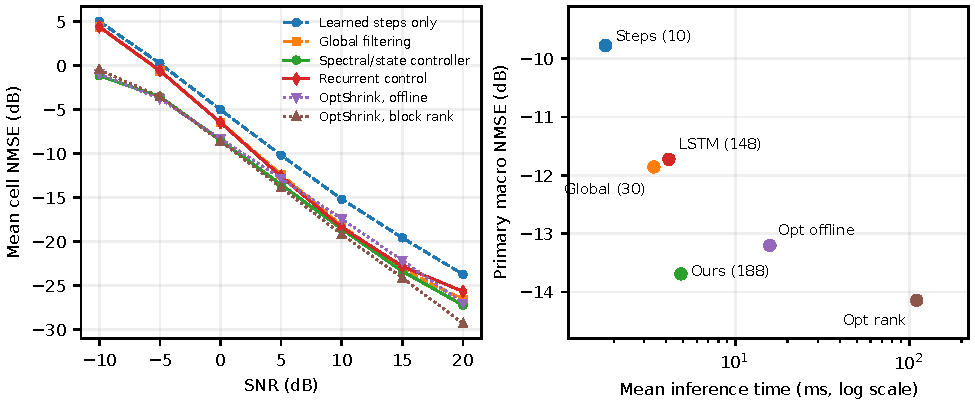
\includegraphics[width=\textwidth]{compact_comparison.pdf}\caption{Fresh compact-control comparison. Left: each SNR point averages 18 reference/path cells. Right: primary accuracy and measured serial inference time. These descriptive summaries do not imply cellwise confidence guarantees.}\label{fig:compact}\end{figure*}



\section{Historical: Training-Recipe Checks and Noise-Input Sensitivity}
\label{sec:training-updates}

The original 188-parameter estimator remains the proposed method. The
checks below change its training recipe or select between two frozen
models; they do not add a new estimator architecture. Each study has its
own fresh test cases. Their numerical averages must not be pooled as if
they came from one experiment. A severe error means per-case channel
NMSE $>1$, not a measured communication outage or numerical divergence.

\subsection{All-Pilot Rician Training}

The original loss estimates a channel from 21 pilot columns and predicts
nine held-out columns. Inference uses all 30 columns. To test this change
in input geometry, we also trained using all pilot columns, following
the re-corruption principle~\cite{pang2021r2r}. For an observed magnitude
$z=|\mu+w|$, with noiseless mean $\mu=(GS+B)_{np}$ and
$w\sim\CN(0,v)$, draw an independent
$\eta\sim\CN(0,v)$ and fix $\alpha>0$. Form
\begin{equation}
 z_{\rm in}=|z+\alpha\eta|,\qquad
 z_{\rm target}=|z-\eta/\alpha|.
\end{equation}
The input and target complex-noise variances are
$v(1+\alpha^2)$ and $v(1+\alpha^{-2})$, respectively. The EM update uses
the first variance, and the predictive Rician loss uses the second.

This construction does not require the unobserved complex field. To
check its distribution, write $Y=\mu+w$ and rotate $\eta$ by $\arg Y$.
Circular symmetry leaves the rotated noise independent of $Y$ and
unchanged in distribution. The resulting complex noises are
$w+\alpha\eta'$ and $w-\eta'/\alpha$. They are jointly proper Gaussian,
with cross-covariance $v-v=0$. Their magnitudes are therefore independent
conditional on $\mu$. They are \emph{not} independent conditional on a
fixed saved magnitude $z$. Repeated artificial corruptions of one block
are augmentations, not new channels. This argument assumes known,
independent circular Gaussian field noise and fixed $\alpha$; it is not
an unbiased-channel-NMSE result. The predictive likelihood and channel
error remain different objectives.

An initial development screen used 2,304 training blocks, 384 validation
blocks, two initialization seeds (10401 and 10402), and ten epochs. Its
six primary cells had SNR $-5,5,15$ dB, RSR $5,12$ dB, and random
3--7 paths per user. The 384 primary test worlds and 128 separate stress
worlds were generated after model freezing. Fixed-final-epoch scores
were primary: original, $\alpha=0.5$, and $\alpha=1$ gave
$-12.392$, $-12.835$, and $-13.365$ dB, with severe rates
$1.562\%$, $0.521\%$, and $0.391\%$. The two seed gains for
$\alpha=0.5$ were $-0.222$ and $1.109$ dB; for $\alpha=1$ they were
$0.747$ and $1.198$ dB. Thus the screen supported testing $\alpha=1$,
not a universal gain or reduced failure rate. Checkpoints selected by
the common 21/9 validation loss were secondary in this small screen.

\subsection{Matched Full-Budget Comparison}

The larger study fixed $\alpha=1$ before generating new test data. It
used the original 16,384 training blocks and 2,048 validation blocks,
three matched initialization seeds (9101--9103), 20 epochs, Adam with
step size $10^{-3}$, and batches of 32. Both learned recipes retained the same
188 parameters and ten EM/filtering stages. New artificial noise was
drawn each epoch. Initialization and epoch data orders matched the
original runs. Matching examples and optimizer updates does not match
training operations, noise distributions, or objectives. The experiment
tests the whole training recipe, not pilot geometry alone; 20 epochs
do not establish convergence.

Both methods' primary checkpoints minimize equal-condition 21/9
validation Rician loss, with epoch zero eligible. This preserves the
original selection rule but may favor its training recipe. Final-epoch
comparisons are reported separately. The full-budget study contains
8,192 fresh worlds in two banks (seeds 20261014211001 and
20261014221001), with 32 cases per cell and bank. Its 126 primary
conditions cross SNR $-10$ to $20$ dB in 5 dB steps, RSR $5,12,20$ dB,
and random 3--7 or fixed $2,4,8,12,16$ paths per user. Here
$N=32$, $K=3$, and $P=30$. Two stress cells add 128 worlds but do not
enter the primary metric. Offline and per-block rank-selected OptShrink
reuse frozen validation choices; per-block selection scores ranks
0--15 on 21/9 columns and refits all 30 columns.

The primary score pools the two banks' squared errors and channel powers
within each cell, takes their dB ratio, averages the 126 cells equally,
then averages the three model-specific scores. This is neither an
ensemble nor the dB of one pooled full-range ratio. All-pilot training
improves this score by $0.277$ dB over the original, but is $0.171$ dB
worse than block-rank OptShrink. It wins 106/126 cells against the
original, with a largest observed loss of $0.527$ dB. Severe errors
increase from $2.819\%$ to $4.473\%$; hence the average improvement is
not a general reliability improvement. The final-epoch gain is
$0.242$ dB. All-pilot training reduces the nearly noiseless error floor
but remains far behind OptShrink there, and does not fix weak-reference
performance. Tables~\ref{tab:training-full}--\ref{tab:training-seeds}
give the sensitivity, uncertainty and training records.

The two declared average-gain intervals use 4,000 paired resamples
within bank/cell, with Bonferroni adjustment. Pairing is retained across
methods and model seeds. The intervals condition on the fitted models
and shared training dataset; three initializations are not three
independent training populations. CPU timings use one PyTorch thread,
float64, batch one, and three randomized repeats per condition. They
include initialization and rank search/refitting, but exclude loading,
file access, and offline fitting. Original and all-pilot inference take
about 4.81 ms, compared with 15.66 ms for offline OptShrink and
108.08 ms for block-rank OptShrink. These are measured implementation
costs, not a hardware-independent complexity claim.

\begin{figure*}[!t]
\centering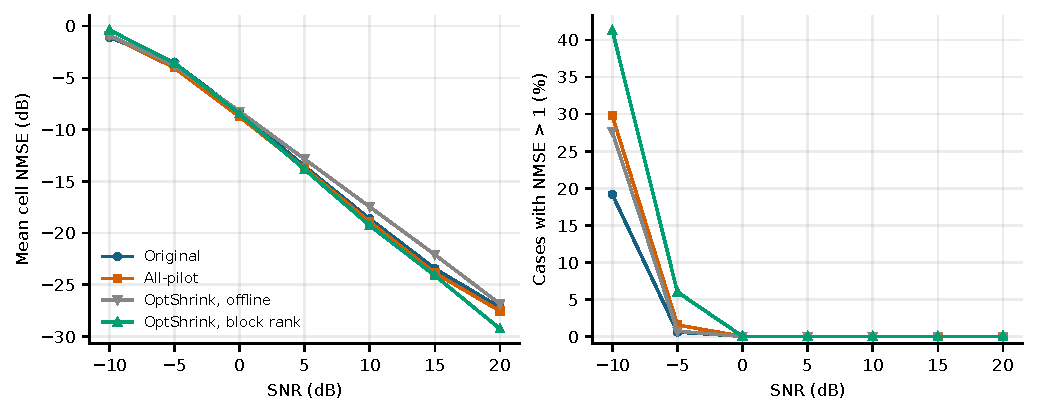
\includegraphics[width=\textwidth]{training_tradeoff.pdf}
\caption{The separate full-budget training comparison. Each SNR averages 18 reference/path conditions. Better average channel accuracy does not imply fewer severe errors. Curves use the same 8,064 primary worlds; neural scores average three fits, not an ensemble.}
\label{fig:training-tradeoff}
\end{figure*}

\subsection{One-Seed Mixed-Training Screen}

A separate test used seed 9101 and the same full training budget, with
exactly half the 512 batches per epoch assigned to each recipe. Each
batch still used one model evaluation and one optimizer update. The
two losses were averaged per measurement and logged separately; their
different noise levels make their raw scales incomparable. The same
21/9 validation rule selected epoch 19. Testing used 4,096 new worlds
(bank 20261015111001), including 4,032 primary and 64 stress worlds.

Mixed training improved the selected original by $0.152$ dB. Its
$0.033$ dB deficit to selected all-pilot training is descriptive: the
adjusted gain interval $[-0.0668,0.0008]$ dB includes zero. Its severe rate was
$3.745\%$, between the original's $2.902\%$ and all-pilot's $4.762\%$.
Compared with all-pilot, it corrected 42 severe outcomes and introduced
one; compared with the original, it introduced 34 and corrected none.
At $-10$ dB it reduced both mean-case error and severe frequency versus
all-pilot. At $-5$ dB it reduced severe frequency but increased mean-case
NMSE by $0.0100$. Its 5.008 ms runtime was only $0.56\%$ above the
original's measured time. Table~\ref{tab:training-mixed} retains all
selected/final results and the matched classical controls.

The predefined screen required a $0.2$ dB gain over the original,
lower mean-case error and severe frequency than all-pilot at both
$-10$ and $-5$ dB, an overall severe-rate increase of at most 0.2
percentage points over the original, and runtime at most $1.05$ times
the original. It passed the severe-frequency and runtime checks, but
failed the gain, low-SNR mean-error, and overall severe-rate checks.
This one-seed development result is not promoted to the main method.
Its 2,000 paired resamples condition on that one fit; only the four
macro-gain contrasts receive multiplicity adjustment. The screening
tolerances are practical rules, not statistical noninferiority claims.

\subsection{Simple Selection and Incorrect Noise Inputs}

We next froze the seed-9101 original and all-pilot models without
retraining. A scalar rule uses nominal SNR $10\log_{10}(3/\widetilde v)$
and selects the original below a threshold and all-pilot above it.
The constant 3 is the known expected signal power under this normalized
three-user benchmark, not the unknown realized channel power. The rule
is not established for arbitrary unknown path loss. Candidate cutoffs
were $-7.5,-2.5,2.5,7.5,12.5,17.5$ dB, plus both constant policies.
Selection used only the 2,048 validation observations, fixed 21/9
prediction loss, and equal condition weights, without channel labels.

Validation selected \emph{always original}: average loss 3.372665,
compared with 3.372740 for the 17.5 dB cutoff and 3.386371 for always
all-pilot. We did not force a switch or revise the cutoff after testing.
The 21/9 criterion may favor the original recipe and need not rank
all-30-pilot channel accuracy identically. This negative result rejects
this particular selection procedure, not every possible selector.

The new bank (20261015151001) has 4,224 worlds: 4,032 primary cases,
64 weak-reference/nearly-noiseless stress cases, and 128 off-grid cases
at SNR $\pm2.5$ dB with RSR 5/12 dB. Each physical observation is reused
with supplied variance $\widetilde v=v10^{\delta/10}$,
$\delta\in\{0,-3,+3\}$ dB. Raw magnitudes, pilots, reference, actual
noise, and true channels remain fixed. Every comparator and the router
receive the same biased variance. The three settings therefore are not
three independent test populations.

Table~\ref{tab:training-noise} shows a substantial sensitivity to noise
underestimation. The original's severe rate rises from $2.803\%$ with
correct variance to $11.111\%$ at $-3$ dB; the all-pilot rate rises
from $4.861\%$ to $14.509\%$. Overestimation by 3 dB gives $3.398\%$
and $5.432\%$, respectively. Because the frozen policy is constant,
there are no route changes and its estimates equal the original's.
The correct-noise $0.1$ dB gain criterion fails, although the severe-rate,
low-SNR and $1.05$ runtime criteria pass. The selector stores 376 model
weights plus the cutoff, evaluates only one 188-parameter model per
case, and takes 4.945 ms versus 4.875 ms for the original. No OptShrink
rerun is included in this screen. Its 2,000 paired intervals are
descriptive, conditional on the two fitted models, and unadjusted.

\subsection{Oracle Phase Diagnostic and Audit Scope}

A separate diagnostic uses 576 new worlds (seed 20261014031001), with
64 per SNR/RSR cell. It evaluates the three frozen original models at
SNR $-5,5,15$ dB and RSR $0,5,12$ dB. The raw, truth-aligned global-phase,
and truth-aligned antenna-row-phase average scores are $-10.833$,
$-10.912$, and $-12.853$ dB. The much larger row-wise change at weak
reference identifies an error component, not an implementable receiver
gain. Alignment can remove noise as well as phase error; it does not
prove a distinct local minimum or a physical reference-drift mechanism.
No learned setting is chosen from this diagnostic.

Saved audits checked paired identifiers, source/data/model hashes,
complete histories, frozen validation choices, finite outputs, and
representative prediction replays. The full-budget study replayed
384 neural and 64 independent classical predictions; mixed training
replayed 60 neural and 20 classical predictions; the selector replayed
1,188 predictions. Maximum neural discrepancies were below
$5\times10^{-15}$. This is not a replay of every training update.
The manuscript material generator independently recomputes primary
NMSE and severe rates from the saved error arrays. Small evidence files
retain all condition-level summaries, protocols, phase diagnostics,
selection scores and input hashes. These checks establish consistency
of the numerical record, not hardware validation, optimality,
convergence, or robustness to new training populations.

\begin{table*}[!t]
\caption{Full-budget study: selected and final-epoch sensitivity, plus separate stress cells. Primary scores use 8,064 worlds; each stress cell has 64 worlds. Weak reference: SNR 5/RSR 0 dB. Nearly noiseless: SNR 60/RSR 12 dB. Stress scores do not enter the primary score.}
\label{tab:training-full}\centering\footnotesize
\setlength{\tabcolsep}{3pt}
\begin{tabular}{@{}lrrrrr@{}}\toprule
Method & Macro (dB) & Pooled (dB) & Severe (\%) & Weak reference & Nearly noiseless\\
\midrule
Original (selected) & -13.684 & -6.650 & 2.82 & -7.244 & -6.949\\
All-pilot (selected) & -13.962 & -6.711 & 4.47 & -6.903 & -15.240\\
Original (final) & -13.762 & -6.684 & 3.04 & -7.280 & -6.921\\
All-pilot (final) & -14.005 & -6.695 & 4.61 & -6.865 & -23.116\\
OptShrink, block rank & -14.132 & -6.201 & 6.76 & -11.257 & -69.517\\
OptShrink, offline & -13.168 & -6.568 & 4.04 & -11.866 & -66.684\\
\bottomrule
\end{tabular}
\end{table*}

\begin{table*}[!t]
\caption{All-pilot gains: positive favors all-pilot training. Two predeclared contrasts, Bonferroni-adjusted conditional 95\% intervals. Worst observed harm is not a confidence bound.}
\label{tab:training-contrasts}\centering\footnotesize
\setlength{\tabcolsep}{3pt}
\begin{tabular}{@{}lrrrr@{}}\toprule
Comparator & Gain (dB) & 95\% interval & Cell wins & Worst harm\\
\midrule
Original (selected) & +0.277 & [+0.263, +0.294] & 106/126 & 0.527\\
OptShrink, block rank & -0.171 & [-0.221, -0.117] & 72/126 & 3.744\\
\bottomrule
\end{tabular}
\end{table*}

\begin{table}[!t]
\caption{Full-budget training records. Seeds share one training dataset. All-pilot training times include validation and concurrent-worker contention; they are not isolated-device benchmarks.}
\label{tab:training-seeds}\centering\footnotesize
\setlength{\tabcolsep}{3pt}
\begin{tabular}{@{}rrrrr@{}}\toprule
Seed & Original & All-pilot & Best epoch & Minutes\\
\midrule
9101 & -13.786 & -13.978 & 16 & 29.05\\
9102 & -13.446 & -13.938 & 18 & 28.99\\
9103 & -13.822 & -13.969 & 17 & 29.31\\
\bottomrule
\end{tabular}
\end{table}

\begin{table*}[!t]
\caption{Separate one-seed mixed-training screen: 4,032 primary worlds, not the full-budget test bank. Mean-case NMSE is linear. Selected-checkpoint comparisons are primary; final checkpoints are sensitivity checks.}
\label{tab:training-mixed}\centering\footnotesize
\setlength{\tabcolsep}{3pt}
\begin{tabular}{@{}lrrrr@{}}\toprule
Method & Macro (dB) & Case mean & Severe (\%) & Time (ms)\\
\midrule
Original (selected) & -13.799 & 0.2222 & 2.90 & 4.98\\
All-pilot (selected) & -13.984 & 0.2200 & 4.76 & 4.96\\
Mixed (selected) & -13.951 & 0.2163 & 3.75 & 5.01\\
Original (final) & -13.672 & 0.2224 & 3.00 & 4.98\\
All-pilot (final) & -14.004 & 0.2209 & 4.96 & 4.96\\
Mixed (final) & -13.966 & 0.2160 & 3.84 & 5.01\\
OptShrink, offline & -13.119 & 0.2257 & 4.69 & 16.06\\
OptShrink, block rank & -14.147 & 0.2454 & 6.70 & 115.20\\
\bottomrule
\end{tabular}
\end{table*}

\begin{table*}[!t]
\caption{Separate one-seed selector/noise-input screen: the same 4,032 primary worlds at all three supplied-variance offsets. Physical observations and actual noise are unchanged. The selected rule always runs the original model.}
\label{tab:training-noise}\centering\footnotesize
\setlength{\tabcolsep}{3pt}
\begin{tabular}{@{}rlrrrr@{}}\toprule
Offset (dB) & Method & Macro (dB) & Case mean & Severe (\%) & Time (ms)\\
\midrule
+0 & Original (selected) & -13.817 & 0.2228 & 2.80 & 4.88\\
+0 & All-pilot (selected) & -14.033 & 0.2207 & 4.86 & 4.86\\
+0 & Selected rule & -13.817 & 0.2228 & 2.80 & 4.95\\
-3 & Original (selected) & -13.195 & 0.4064 & 11.11 & 4.85\\
-3 & All-pilot (selected) & -13.007 & 0.4962 & 14.51 & 4.85\\
-3 & Selected rule & -13.195 & 0.4064 & 11.11 & 4.94\\
+3 & Original (selected) & -13.228 & 0.2652 & 3.40 & 4.86\\
+3 & All-pilot (selected) & -13.781 & 0.2448 & 5.43 & 4.88\\
+3 & Selected rule & -13.228 & 0.2652 & 3.40 & 4.94\\
\bottomrule
\end{tabular}
\end{table*}

\begin{table*}[!t]
\caption{Separate phase diagnostic: 64 worlds per cell, averaged across three original fitted models. Both aligned scores use the true channel and are oracle-only, not receiver performance. Last column is the fraction of squared error removed by row-wise alignment.}
\label{tab:training-phase}\centering\footnotesize
\setlength{\tabcolsep}{3pt}
\begin{tabular}{@{}rrrrrr@{}}\toprule
SNR & RSR & Raw (dB) & Global oracle & Row oracle & Removed (\%)\\
\midrule
-5 & 0 & 0.366 & 0.296 & -2.176 & 44.2\\
-5 & 5 & -2.184 & -2.263 & -2.932 & 15.8\\
-5 & 12 & -4.288 & -4.331 & -4.820 & 11.5\\
5 & 0 & -7.110 & -7.270 & -11.051 & 59.6\\
5 & 5 & -13.761 & -13.834 & -14.705 & 19.5\\
5 & 12 & -14.012 & -14.071 & -14.786 & 16.3\\
15 & 0 & -8.306 & -8.386 & -15.192 & 79.5\\
15 & 5 & -23.972 & -24.078 & -25.005 & 21.2\\
15 & 12 & -24.226 & -24.269 & -25.007 & 16.5\\
\bottomrule
\end{tabular}
\end{table*}



\section{Historical: Broad OptShrink Comparisons: Full Numerical Record}

Study A tunes OptShrink on the original 2,048 validation observations and masks. Study B inherits that lookup and selects rank from each new block of observations. Neither study retrains the compact estimator. Each has two independent test banks, 126 primary cells and two separate stress cells. All 30 pilots are reused for the final fit, without additional observations. The inference lookup uses supplied noise and reference strength, not true channel power or path count.

Study A uses test-bank seeds 202610210001 and 202610310001; Study B uses 202610610001 and 202610710001. Each cell adds 100 times its zero-based index to the bank seed. Both use 16 worlds per cell and bank. The selected-model seeds are 9101, 9102 and 9103. Sources, settings and checkpoints are hashed before test generation. Settings remain frozen after the test data are inspected.

The primary score averages 126 per-cell dB ratio-of-sums NMSE values, after pooling the two equal-sized test banks within each cell. It is not the dB of one pooled error ratio. Learned scores average the three separate model scores. Bootstrap resampling preserves pairing within each bank/cell; confidence intervals condition on these weights and the offline validation choices. They do not cover repeated training or offline selection uncertainty.

\subsection{Declared Contrasts and All Comparators}

The numerical tables separate the declared average-dB contrasts, alternative error summaries, individual models, test banks and stress cases. These summaries are not interchangeable: a gain in one average does not establish a gain in every cell or at every error threshold. All individual-cell scores are retained in the evidence records.

\begin{table*}[!t]
\caption{Learned gain (positive favors learning), three-contrast-adjusted 95\% intervals within each study, and largest observed primary-cell deterioration. Cellwise safety is not established.}
\label{tab:broad-ci}\centering\footnotesize
\setlength{\tabcolsep}{4pt}
\begin{tabular}{@{}llrrr@{}}\toprule
Study & Comparator & Gain (dB) & Adjusted interval & Worst harm (dB)\\
\midrule
A & Offline OptShrink, selected placement & 0.537 & [0.450, 0.695] & 3.117\\
A & Offline OptShrink, in-loop & 0.565 & [0.477, 0.723] & 3.117\\
A & Offline OptShrink, final-only & 0.738 & [0.621, 0.925] & 3.686\\
B & Online rank + placement selection & -0.449 & [-0.569, -0.358] & 4.478\\
B & Online rank, in-loop & -0.507 & [-0.562, -0.437] & 5.495\\
B & Online rank, final-only & -0.076 & [-0.226, 0.025] & 3.445\\
\bottomrule
\end{tabular}
\end{table*}


\begin{table}[!t]
\caption{Study A: all primary averages and mean end-to-end CPU time. Fixed-budget labels denote EM updates, not matched runtime.}
\label{tab:all-A}\centering\footnotesize
\setlength{\tabcolsep}{4pt}
\begin{tabular}{@{}lrr@{}}\toprule
Method & NMSE (dB) & Time (ms)\\
\midrule
Offline OptShrink, selected placement & -13.028 & 15.61\\
Offline OptShrink, in-loop & -13.000 & 15.57\\
Offline OptShrink, final-only & -12.827 & 6.16\\
OptShrink, 5 updates & -9.816 & 2.47\\
OptShrink, 10 updates & -12.336 & 4.56\\
OptShrink, 20 updates & -12.926 & 8.73\\
OptShrink, 50 updates & -12.941 & 21.20\\
OptShrink, 100 updates & -12.951 & 41.88\\
Original narrow OptShrink lookup & -11.880 & 6.31\\
EM-GS, 100 updates & -9.922 & 13.08\\
HS-Rician, one sweep & -12.996 & 98.91\\
Compact estimator (188 weights) & -13.565 & 4.90\\
\bottomrule
\end{tabular}
\end{table}


\begin{table}[!t]
\caption{Study B: all primary averages and mean end-to-end CPU time. Fixed-budget labels denote EM updates, not matched runtime.}
\label{tab:all-B}\centering\footnotesize
\setlength{\tabcolsep}{4pt}
\begin{tabular}{@{}lrr@{}}\toprule
Method & NMSE (dB) & Time (ms)\\
\midrule
Online rank, in-loop & -14.154 & 108.70\\
Online rank, final-only & -13.723 & 13.96\\
Online rank + placement selection & -14.096 & 114.17\\
Offline OptShrink, selected placement & -13.196 & 15.76\\
Offline OptShrink, in-loop & -13.151 & 15.68\\
Offline OptShrink, final-only & -12.863 & 6.23\\
Original narrow OptShrink lookup & -12.041 & 6.38\\
EM-GS, 100 updates & -9.958 & 13.15\\
HS-Rician, one sweep & -13.059 & 99.88\\
Compact estimator (188 weights) & -13.647 & 4.96\\
\bottomrule
\end{tabular}
\end{table}


\begin{table*}[!t]
\caption{Alternative summaries on primary worlds. Pooled NMSE is in dB; per-case mean NMSE is linear. Last three columns are percentages above the fixed thresholds. Zero observed exceedances do not imply zero population risk.}
\label{tab:broad-tails}\centering\footnotesize
\setlength{\tabcolsep}{4pt}
\begin{tabular}{@{}llrrrrr@{}}\toprule
Study & Method & Pooled & Case mean & $>0.5$ & $>1$ & $>2$\\
\midrule
A & Compact estimator (188 weights) & -6.704 & 0.221 & 19.54 & 3.03 & 0.00\\
A & Offline OptShrink, selected placement & -6.588 & 0.227 & 19.12 & 4.34 & 0.00\\
A & HS-Rician, one sweep & -4.216 & 0.399 & 24.48 & 15.23 & 4.37\\
A & EM-GS, 100 updates & -1.415 & 0.777 & 30.38 & 23.59 & 14.71\\
B & Compact estimator (188 weights) & -6.683 & 0.221 & 19.55 & 3.08 & 0.00\\
B & Online rank, in-loop & -6.217 & 0.247 & 19.52 & 6.87 & 0.22\\
B & HS-Rician, one sweep & -4.166 & 0.402 & 24.50 & 15.48 & 5.21\\
B & EM-GS, 100 updates & -1.392 & 0.778 & 30.63 & 23.26 & 14.96\\
\bottomrule
\end{tabular}
\end{table*}


\begin{figure*}[!t]
\centering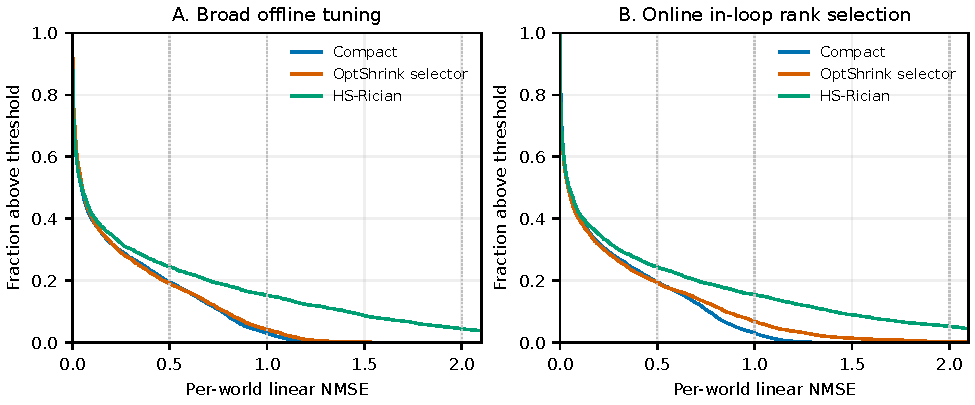
\includegraphics[width=\textwidth]{latest_distributions.pdf}
\caption{Primary empirical exceedance curves over the displayed threshold range, separately by study. Learned curves average the three model-specific empirical distributions on the same worlds; predictions are not independent channels. All values, including larger errors, are retained in the evidence arrays. A lower rate at one threshold does not imply a lower rate at every threshold.}
\end{figure*}
\begin{figure}[!t]
\centering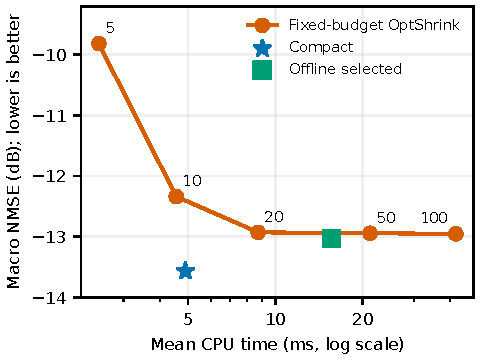
\includegraphics[width=\columnwidth]{latest_cost.pdf}
\caption{Study A accuracy--cost curve. Labels are fixed update budgets, each tuned separately for placement, rank and mixing. The selected lookup may use different budgets by noise/reference pair. No equal-runtime optimum is claimed.}
\end{figure}

\begin{table*}[!t]
\caption{Training-seed and test-bank summaries, kept distinct. Bank dB scores need not average to the score obtained after pooling their linear errors.}
\label{tab:broad-seeds}\centering\footnotesize
\setlength{\tabcolsep}{4pt}
\begin{tabular}{@{}llr@{}}\toprule
Study & Subset & NMSE (dB)\\
\midrule
A & Model 9101 & -13.676\\
A & Model 9102 & -13.327\\
A & Model 9103 & -13.692\\
A & Compact estimator (188 weights), bank 1 & -13.700\\
A & Compact estimator (188 weights), bank 2 & -13.559\\
A & Offline OptShrink, selected placement, bank 1 & -13.059\\
A & Offline OptShrink, selected placement, bank 2 & -13.064\\
B & Model 9101 & -13.759\\
B & Model 9102 & -13.417\\
B & Model 9103 & -13.765\\
B & Compact estimator (188 weights), bank 1 & -13.666\\
B & Compact estimator (188 weights), bank 2 & -13.648\\
B & Offline OptShrink, selected placement, bank 1 & -13.207\\
B & Offline OptShrink, selected placement, bank 2 & -13.183\\
B & Online rank + placement selection, bank 1 & -14.196\\
B & Online rank + placement selection, bank 2 & -14.050\\
B & Online rank, in-loop, bank 1 & -14.166\\
B & Online rank, in-loop, bank 2 & -14.149\\
\bottomrule
\end{tabular}
\end{table*}


\begin{table}[!t]
\caption{Study A: descriptive marginal averages over the other primary conditions. OptShrink is offline-selected. These are not additional independent tests.}
\label{tab:marginal-A}\centering\footnotesize
\setlength{\tabcolsep}{4pt}
\begin{tabular}{@{}llrrr@{}}\toprule
Study & Condition & Compact & OptShrink & Gain\\
\midrule
A & SNR -10 & -1.057 & -0.835 & 0.222\\
A & SNR -5 & -3.682 & -3.894 & -0.212\\
A & SNR 0 & -8.346 & -8.220 & 0.126\\
A & SNR 5 & -13.481 & -12.832 & 0.649\\
A & SNR 10 & -18.636 & -17.375 & 1.262\\
A & SNR 15 & -23.521 & -22.275 & 1.246\\
A & SNR 20 & -26.232 & -25.767 & 0.465\\
A & RSR 5 & -12.494 & -11.840 & 0.654\\
A & RSR 12 & -13.968 & -13.450 & 0.518\\
A & RSR 20 & -14.234 & -13.795 & 0.439\\
A & Paths 3--7 & -14.295 & -13.536 & 0.759\\
A & Paths 2 & -15.863 & -13.674 & 2.190\\
A & Paths 4 & -14.704 & -13.814 & 0.890\\
A & Paths 8 & -13.099 & -13.255 & -0.156\\
A & Paths 12 & -12.119 & -12.309 & -0.190\\
A & Paths 16 & -11.310 & -11.582 & -0.272\\
\bottomrule
\end{tabular}
\end{table}


\begin{table}[!t]
\caption{Study B: descriptive marginal averages over the other primary conditions. OptShrink is online in-loop rank selection. These are not additional independent tests.}
\label{tab:marginal-B}\centering\footnotesize
\setlength{\tabcolsep}{4pt}
\begin{tabular}{@{}llrrr@{}}\toprule
Study & Condition & Compact & OptShrink & Gain\\
\midrule
B & SNR -10 & -1.073 & -0.362 & 0.710\\
B & SNR -5 & -3.605 & -3.574 & 0.031\\
B & SNR 0 & -8.284 & -8.426 & -0.142\\
B & SNR 5 & -13.581 & -13.888 & -0.307\\
B & SNR 10 & -18.694 & -19.289 & -0.595\\
B & SNR 15 & -23.365 & -24.210 & -0.845\\
B & SNR 20 & -26.926 & -29.329 & -2.403\\
B & RSR 5 & -12.754 & -13.098 & -0.345\\
B & RSR 12 & -13.985 & -14.530 & -0.544\\
B & RSR 20 & -14.202 & -14.834 & -0.632\\
B & Paths 3--7 & -14.342 & -14.546 & -0.203\\
B & Paths 2 & -16.436 & -17.151 & -0.715\\
B & Paths 4 & -14.653 & -15.150 & -0.498\\
B & Paths 8 & -13.014 & -13.495 & -0.482\\
B & Paths 12 & -12.210 & -12.592 & -0.382\\
B & Paths 16 & -11.227 & -11.990 & -0.763\\
\bottomrule
\end{tabular}
\end{table}


\begin{table*}[!t]
\caption{Stress conditions, excluded from primary averages. Weak reference: SNR 5/RSR 0 dB. Nearly noiseless: SNR 60/RSR 12 dB. Both use random three-to-seven-path channels.}
\label{tab:broad-stress}\centering\footnotesize
\setlength{\tabcolsep}{4pt}
\begin{tabular}{@{}lllr@{}}\toprule
Study & Condition & Method & NMSE (dB)\\
\midrule
A & Weak reference & Compact estimator (188 weights) & -7.842\\
A & Weak reference & Offline OptShrink, selected placement & -11.905\\
A & Weak reference & EM-GS, 100 updates & -6.109\\
A & Nearly noiseless & Compact estimator (188 weights) & -6.693\\
A & Nearly noiseless & Offline OptShrink, selected placement & -66.886\\
A & Nearly noiseless & EM-GS, 100 updates & -65.604\\
B & Weak reference & Compact estimator (188 weights) & -7.787\\
B & Weak reference & Offline OptShrink, selected placement & -11.498\\
B & Weak reference & EM-GS, 100 updates & -6.261\\
B & Weak reference & Online rank + placement selection & -10.101\\
B & Weak reference & Online rank, in-loop & -10.101\\
B & Nearly noiseless & Compact estimator (188 weights) & -6.835\\
B & Nearly noiseless & Offline OptShrink, selected placement & -67.618\\
B & Nearly noiseless & EM-GS, 100 updates & -66.212\\
B & Nearly noiseless & Online rank + placement selection & -70.134\\
B & Nearly noiseless & Online rank, in-loop & -70.121\\
\bottomrule
\end{tabular}
\end{table*}


\subsection{Frozen Settings and Numerical Verification}

The online selector searches a shared rank, not separate ranks for each user. Its mixing strength and iteration count are inherited from the matching in-loop or final-only row in the offline lookup. Thus the rank comparison does not exhaust all possible classical policies. Candidate initialization uses only the first 21 pilots. After scoring the other nine, the winner starts again from all 30. Joint selection evaluates both placements and counts both searches in timing. Search work shared while generating several experimental arms is not used to understate standalone timing.

\begin{table*}[!t]
\caption{Broad offline settings. Within each placement, columns give rank, mixing factor and update count. The selected column chooses between those placements. Rank zero denotes no filtering.}
\label{tab:settings-broad}\centering\footnotesize
\setlength{\tabcolsep}{4pt}
\begin{tabular}{@{}lrrrrrrl@{}}\toprule
SNR / RSR & Loop $r$ & $\beta$ & $T$ & Final $r$ & $\beta$ & $T$ & Selected\\
\midrule
-10 / 5 & 1 & 0.75 & 5 & 2 & 1.0 & 50 & final\\
-10 / 12 & 1 & 0.5 & 5 & 1 & 0.75 & 5 & final\\
-10 / 20 & 1 & 0.75 & 5 & 1 & 0.75 & 5 & loop\\
-5 / 5 & 2 & 0.5 & 10 & 3 & 0.75 & 20 & final\\
-5 / 12 & 2 & 0.5 & 5 & 2 & 0.75 & 5 & loop\\
-5 / 20 & 3 & 0.75 & 5 & 3 & 0.75 & 5 & loop\\
0 / 5 & 4 & 0.5 & 20 & 5 & 0.75 & 100 & loop\\
0 / 12 & 4 & 0.5 & 10 & 5 & 0.75 & 10 & loop\\
0 / 20 & 4 & 0.5 & 10 & 7 & 1.0 & 5 & loop\\
5 / 5 & 7 & 0.5 & 100 & 8 & 1.0 & 100 & loop\\
5 / 12 & 7 & 0.5 & 20 & 8 & 1.0 & 20 & loop\\
5 / 20 & 8 & 0.75 & 10 & 8 & 1.0 & 10 & loop\\
10 / 5 & 9 & 1.0 & 100 & 9 & 0.75 & 100 & loop\\
10 / 12 & 10 & 0.75 & 20 & 9 & 1.0 & 50 & loop\\
10 / 20 & 10 & 1.0 & 20 & 10 & 1.0 & 20 & loop\\
15 / 5 & 9 & 0.5 & 50 & 10 & 1.0 & 100 & loop\\
15 / 12 & 10 & 0.75 & 50 & 10 & 1.0 & 50 & loop\\
15 / 20 & 10 & 0.75 & 50 & 10 & 1.0 & 50 & loop\\
20 / 5 & 11 & 1.0 & 100 & 13 & 1.0 & 100 & loop\\
20 / 12 & 12 & 1.0 & 50 & 12 & 1.0 & 50 & loop\\
20 / 20 & 11 & 0.75 & 50 & 11 & 1.0 & 50 & loop\\
\bottomrule
\end{tabular}
\end{table*}


Study A: all 4,096 test worlds regenerated exactly; 3,584 representative predictions replayed. Maximum recorded independent classical absolute output difference was $5.73\times10^{-13}$. An independent scalar-loop calculation reproduced every primary score. These checks test the saved implementation and data, not an external reproduction of the study.

Study B: all 4,096 test worlds regenerated exactly; 2,816 representative predictions replayed. Maximum recorded independent rank-selector absolute output difference was $1.26\times10^{-12}$. An independent scalar-loop calculation reproduced every primary score. These checks test the saved implementation and data, not an external reproduction of the study.

Study A also regenerated all 2,048 validation observations and replayed selection from saved scores. Study B independently checked both rank-score vectors, chosen settings and all-pilot refits with NumPy/SciPy. Its new audit did not independently replay HS-Rician again; that backend check is in Study A. Both studies passed finite-output, source-hash, checkpoint-hash and freeze-before-generation checks. No failed trial was removed. Full per-cell values and source records are supplied as JSON evidence in the manuscript archive; full observation and prediction arrays remain in the experimental archive.


\section{Historical: Retained Negative Follow-Ups}
These studies tested possible improvements before the broad comparisons.
None changed the three original 188-parameter checkpoints. Their outcomes
are kept separate because they use different test banks and budgets.

\subsection{A Controller Around OptShrink}
The first hybrid used a learned mixing rule around OptShrink. On 704 fresh
worlds, its seven-SNR average was $-14.129$~dB, compared with
$-14.535$~dB for the stronger OptShrink control. It therefore lost
0.406~dB. Its ten-stage schedule and some ranks did not match the strong
baseline. A clipped gate also had zero local derivative in many high-SNR
cases. These were reasons to repair the comparison, not evidence that
repairing it would produce an improvement.

The corrected pilot used the strong baseline's ranks and noise-dependent
iteration schedule, removed the hard clipping, and trained two
initializations on one shared dataset. Settings were fixed before 704 new
test worlds were generated. The learned gate started at 0.95 where the
baseline used strength one; a near-initial control accounted for this
difference. Table~\ref{tab:hybrid-retained} gives the primary seven-SNR
averages. Four stress cells were reported separately.

\begin{table}[!t]
\caption{Corrected hybrid pilot: lower NMSE is better.}
\label{tab:hybrid-retained}\centering\small
\begin{tabular}{@{}lr@{}}\toprule
Method & NMSE (dB)\\\midrule
Strong OptShrink & $-14.596$\\
Retuned classical mixing & $-14.637$\\
Residual-based classical rule & $-14.633$\\
Stage-only learned mixing & $-14.656$\\
Corrected measurement-conditioned hybrid & $-14.616$\\\bottomrule
\end{tabular}
\end{table}

The corrected hybrid gained only 0.019~dB over the strong starting
baseline, with conditional pointwise 95\% interval
$[0.004,0.033]$~dB. It lost 0.022~dB to retuned classical mixing and
0.040~dB to the simpler stage-only learned rule. Mean same-backend
processing times were about 7.2~ms for the hybrid and 6.2~ms for
OptShrink. The corrected gate had no exact-zero local slopes in the
recorded tests, but this did not make it the better estimator. The
screen failed, and the hybrid was not expanded. Its numerical audit
regenerated 2,720 worlds and checked 198 checkpoint predictions and
11 independent classical predictions.

\subsection{Stopping, Filter Release and a Larger Learned Control}
A separate 704-world pilot included two independent 352-world banks,
each with 32 worlds in seven primary and four stress cells. The first
bank tested observable stopping and releasing the structural filter.
Frozen OptShrink, observed stopping and observed release reached
$-14.530$, $-14.498$ and $-14.449$~dB, respectively. Release lost
0.050~dB to observed stopping and 0.081~dB to frozen OptShrink. Stopping
improved the weak-reference diagnostic, but not the primary average.
It computed all 100 updates before choosing an output; its selected
iteration count was not its total processing cost.

The second bank compared a newly trained compact model with an
independently implemented exact-EM Transformer with 1,585,920 parameters.
Both used 4,096 training cases, 12 epochs, matching masks and order,
one training seed, and held-out likelihood for selection. Selected
NMSEs were $-14.325$~dB for the compact model, $-9.726$~dB for the
Transformer, $-14.289$~dB for OptShrink and $-10.116$~dB for EM100.
The compact--OptShrink gain interval, $[-0.095,0.176]$~dB, included zero.
The Transformer was worse than EM100, so this pilot did not provide a
strong learned comparator. It was not a reproduction of published
URformer and supports no superiority claim over that method. Neither
training budget establishes convergence.

\subsection{An Error-Model Feasibility Check}
A further screen examined whether local sensitivity could predict the
error entering a Hankel filter. It used 24 fixed channel/pilot/reference
worlds, 256 repeated noise draws and eight separate prediction anchors
per world. Noise repetitions were not new channel realizations. The
ordinary-start covariance check passed six of ten primary groups,
below its required eight; the total-error/bias check passed seven.
At SNR $-10$~dB after 100 EM updates, predicted variance was 16.48
times observed variance. With a weak reference it was 5.72 times.
Estimated bias accounted for about 57\% of total error at 20 updates
and 22\% at 100 updates in the weak-reference group.

Two supplementary finite-difference checks exceeded their original
tolerance. Smaller steps and independent automatic differentiation
resolved the numerical discrepancy. Ordinary-start relative Jacobian
errors in the two problematic settings were about 0.0113\% and
0.0023\%, too small to explain the main prediction failure. The
scientific screen remained failed. This study concerned unfiltered,
row-separable EM; it did not validate an error model for interleaved
Hankel reconstruction or establish an optimal shrinker. No new filter
was promoted on the basis of these predictions.

\subsection{What These Checks Leave Open}
An observable likelihood score is not a channel-error guarantee. A
smooth gate is not enough to establish useful adaptation. More network
parameters do not establish a stronger trained baseline. The retained
failures narrow the claim to the tested original compact estimator;
they do not supply evidence for a new hybrid, an uncertainty-aware
filter or a general improvement to OptShrink.

\subsection{Retained Figures From the Earlier Studies}
These plots retain the earlier narrow-population and operating-limit
results. They use the protocols stated in their captions, not the
new broad-study test banks.
\begin{figure*}[!t]
\centering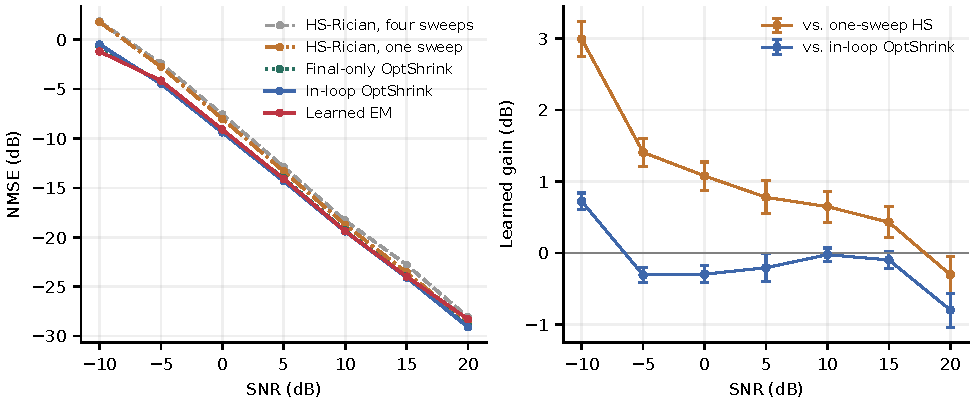
\includegraphics[width=\textwidth]{optshrink.pdf}
\caption{Earlier narrow-population comparison: 128 paired trials per SNR
and frozen learned models. The one-sweep HS-Rician result was added on
the same saved worlds. Right: learned gains over one-sweep HS-Rician
and in-loop OptShrink; positive favors learning. Intervals are pointwise
and condition on the saved models.}
\end{figure*}
\begin{figure*}[!t]
\centering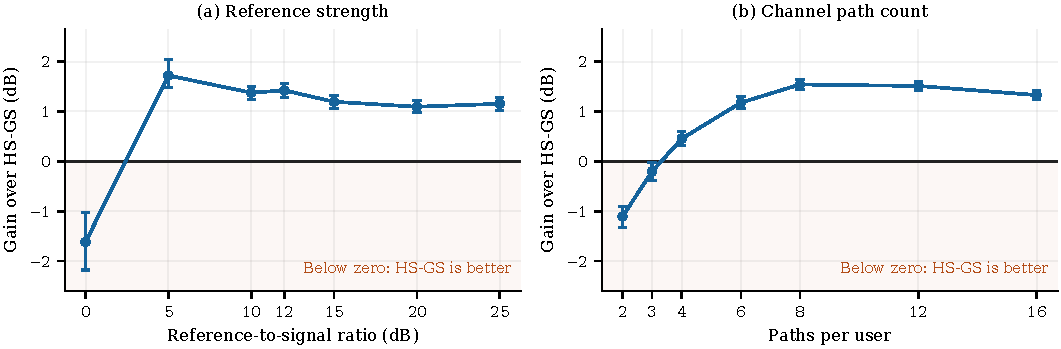
\includegraphics[width=\textwidth]{learned_limits.pdf}
\caption{Limits in the original learned study at SNR 5~dB.
(a) Reference strength for three-to-seven-path channels.
(b) Fixed path counts at RSR 12~dB. Gains compare adaptive EM with
four-sweep HS-amplitude (HS-GS in the plot). Bars are conditional
pointwise paired intervals; tested path counts overlap training.}
\end{figure*}


\input{merged_followup.tex}

\section{Historical: Local Recovery and Reference Calibration}
For one array element, let $g,s_p\in\mathbb C^K$, with
$\mu_p=g^Ts_p+b_p$ and noiseless amplitude $a_p=|\mu_p|$.
Use real coordinates $x=[\operatorname{Re}g^T,\operatorname{Im}g^T]^T$.
When every $\mu_p\ne0$, differentiation gives
\begin{align}
 da_p&=\operatorname{Re}\{\mu_p^*s_p^T dg/|\mu_p|\},\\
 A_p&=[\operatorname{Re}c_p^T,-\operatorname{Im}c_p^T],\qquad
 c_p=\mu_p^*s_p/|\mu_p|.
\end{align}
Here $A\in\R^{P\times2K}$ is the real amplitude Jacobian.

\textit{Local statement.} If $\rank A=2K$, the noiseless amplitude map
is one-to-one in a sufficiently small neighborhood of this $g$.
To see this, choose $2K$ independent rows. Their square Jacobian is
invertible, so the inverse-function theorem supplies a local inverse for
that measurement subset. The remaining measurements cannot remove this
local injectivity. This is not a global uniqueness theorem: distant
channels may give the same measurements. A rank-deficient Jacobian also
does not, by itself, rule out all forms of nonlinear local injectivity.

For small perturbations at a full-rank point, least-squares inversion has
first-order sensitivity bounded by $1/\sigma_{\min}(A)$.
Thus $P\ge2K$ is necessary for regular full-rank local recovery of an
unrestricted row. It is not sufficient. Full row rank of $S$ permits
the EM linear solve but does not ensure full rank of $A$. These are
standard local arguments in an affine phase-retrieval setting, not a new
identifiability theorem~\cite{gao2018}. Sparse channel constraints require their own
parameterization and Jacobian; a path-count condition is not derived here.

\subsection{Rician Information}
For known complex variance $v>0$ and $a>0$, the amplitude score is
\begin{equation}
 h(z,a,v)=-2a/v+(2z/v)I_1(2za/v)/I_0(2za/v).
\end{equation}
Define $w(a,v)=\mathbb E[h(Z,a,v)^2]$, with expectation under the
Rician observation law. For independent pilots the real Fisher matrix is
\begin{equation}
 J=A^T\diag\{w(a_p,v)\}_{p=1}^P A.
\end{equation}
Each magnitude observation contributes an outer product of rank at most one, not a
full-rank complex information block. For finite $v>0$ and nonzero
amplitudes these weights are positive. At a zero field the regular
amplitude-coordinate derivation is not used; first-order information
about the Cartesian mean vanishes. When the assumptions hold, the
rank and conditioning of $J$ give a local diagnostic. Neither a small
bound nor a well-conditioned matrix at the true channel guarantees that
an iterative estimator reaches the correct solution.

\subsection{What a Reference Does and Does Not Fix}
With $B=0$, $g$ and $e^{j\phi}g$ have identical amplitudes for every
$\phi$. The Jacobian has the phase direction $jg$ in its null space for
nonzero $g$. A nonzero known reference can remove that symmetry, but
arbitrary reference and pilot patterns still require a rank check. For
example, if $b_p=c^Ts_p$ for some fixed $c$, then
$g'=e^{j\phi}(g+c)-c$ produces the same amplitudes. This can occur
with a full-row-rank pilot matrix and a nonzero reference.
RSR $0$~dB in our experiments means a nonzero reference equal in expected
power to one user; it is not the absent-reference case.

There is a separate calibration ambiguity. If the estimator assumes
$B'=e^{j\phi}B$, then $G'=e^{j\phi}G$ gives
\begin{equation}
 |G'S+B'|=|e^{j\phi}(GS+B)|=|GS+B|.
\end{equation}
The likelihood therefore cannot identify a constant reference-phase error
from these observations alone. With error measured in the original
reference frame, even this otherwise exact rotated estimate has NMSE
$|e^{j\phi}-1|^2=4\sin^2(\phi/2)$. At $10^\circ$ this is about
$0.0304$ ($-15.2$~dB). This is an illustrative exact-fit ambiguity, not
a lower bound on every biased estimator. A smaller withheld loss cannot
certify correct absolute phase or recover an unknown reference phase.
Time-varying phase errors generally cannot be absorbed into one constant
channel rotation. A separate static calibration diagnostic estimates a
shared positive amplitude multiplier and noise variance under stated
assumptions. It cannot remove this unknown-phase ambiguity.

\section{Historical: Filter Properties and Computation}
Let $H=U\diag(\sigma_i)V^H\in\mathbb C^{m\times q}$, $m\ge q$, and
\begin{equation}
 F_\tau(H)=H-\tau^2H(H^HH+\tau^2I)^{-1},\qquad\tau>0.
\end{equation}
Its singular values are $f_\tau(\sigma)=\sigma^3/(\sigma^2+\tau^2)$.
Thus $0\le f_\tau(\sigma)\le\sigma$ and
\begin{equation}
 \|F_\tau(H)\|_F\le\|H\|_F,\qquad
 \|F_\tau(H)-H\|_F\le\sqrt q\,\tau/2.
\end{equation}
The second inequality follows because
$\sigma-f_\tau(\sigma)=\sigma\tau^2/(\sigma^2+\tau^2)\le\tau/2$.

For a channel vector, let $d_i$ count its occurrences in the Hankel
matrix and define $\|g\|_D^2=\sum_i d_i|g_i|^2=\|\Hank(g)\|_F^2$.
Antidiagonal averaging followed by lifting is the orthogonal projection
onto Hankel matrices in Frobenius norm. Therefore for fixed realized
$\eta\in[0,1]$ and $\tau>0$,
\begin{align}
 g^+&=(1-\eta)g+\eta\Hank^\dagger F_\tau(\Hank(g)),\\
 \|g^+\|_D&\le\|g\|_D,\qquad
 \|g^+-g\|_D\le\eta\sqrt q\,\tau/2.
\end{align}
This bounds the size of one correction, not its error relative to the
unknown true channel. It does not prove a contraction between two
different inputs, particularly when the controller changes $\eta$ and
$\tau$ with the input. It also does not prove convergence of the full
estimator. For fixed $H$, $\tau\to0$ gives $F_\tau(H)\to H$ and
$\tau\to\infty$ gives zero. No low-noise limit is asserted because
the learned threshold need not vanish with noise.

The matrix-solve shrinker is smooth for $\tau>0$, including repeated
singular values. However, the controller also uses ordered largest and
tail singular values. These features need not be differentiable at every
singular-value tie. Finite-gradient numerical checks do not establish
global differentiability of the whole network.

\subsection{Why the Rician Measurement Update Is an EM Step}
Let the unobserved complex field be $Y=GS+B+W$ and write each entry as
$Y_{np}=Z_{np}e^{j\Phi_{np}}$. The receiver observes $Z$, not the phase
$\Phi$. For a current predicted field $M$, the conditional phase density is
\begin{equation}
 p(\phi\mid z,M)=\frac{\exp\{\kappa\cos(\phi-\arg M)\}}
 {2\pi I_0(\kappa)},\qquad \kappa=2z|M|/v.
\end{equation}
This is a von Mises distribution. Its first circular moment gives
\begin{equation}
 Q=\mathbb E[Y\mid Z,M]=Z\frac{I_1(\kappa)}{I_0(\kappa)}e^{j\arg M}.
\end{equation}
At $M=0$, the phase is uniform and $Q=0$. These are conditional complex
fields, not estimates of the mean magnitude. Since $|Y|^2=Z^2$ when $Z$
is fixed, expanding $\mathbb E[\|Y-GS-B\|_F^2\mid Z,M]$ leaves
$\|GS+B-Q\|_F^2$ plus terms independent of the candidate $G$.
Least squares therefore gives $(Q-B)S^H(SS^H)^{-1}$. This derivation uses
independent proper complex Gaussian noise and a supplied positive variance;
it does not use a strong-reference or high-SNR approximation.

\subsection{Relaxed EM Is Not the Same as the Full Stage}
For fixed posterior field $Q$ and supplied variance $v>0$, the negative
EM surrogate, up to constants, is
$\Psi(G)=\|GS+B-Q\|_F^2/v$. Its minimizer is $G_{\rm EM}$ when $S$
has full row rank. The normal equations give
\begin{equation}
 \Psi(G)-\Psi(G_{\rm EM})=\|(G-G_{\rm EM})S\|_F^2/v.
\end{equation}
For $G_\gamma=G+\gamma(G_{\rm EM}-G)$, the surrogate decrease is
\begin{equation}
 \Psi(G)-\Psi(G_\gamma)=\gamma(2-\gamma)
 \|(G-G_{\rm EM})S\|_F^2/v\ge0
\end{equation}
for $0\le\gamma\le2$. Thus even an over-relaxed step within this
interval is a generalized EM step for this quadratic M-step, in exact
arithmetic. The supplied-model likelihood is nondecreasing. This result
does not extend automatically to the subsequent Hankel correction, nor
does it guarantee channel-error reduction, global recovery or convergence
of the complete learned estimator. The secondary GD core is not covered
by this particular argument.

\subsection{Operation Counts}
For $S\in\mathbb C^{K\times P}$ and $G\in\mathbb C^{N\times K}$,
forming $SS^H$ costs $O(K^2P)$. Spectral initialization forms $N$
weighted $(K+1)$-dimensional Gram matrices and eigendecompositions,
costing $O(NP(K+1)^2+N(K+1)^3)$. These are per observation case,
not per stage. The inverse-trace noise proxy adds $O(K^3)$ once.

\begin{table}[!t]
\caption{Leading work per stage, excluding initialization}
\centering\small
\begin{tabular}{@{}p{.47\columnwidth}p{.46\columnwidth}@{}}\toprule
Operation & Leading order\\\midrule
Predicted fields and EM products & $O(NKP)$\\
EM solve, current implementation & $O(NK^2+K^3)$\\
Spectral controller features & $O(Kmq^2)$\\
Smooth matrix filter & $O(Kmq^2+Kq^3)$\\
Antidiagonal averaging & $O(Kmq)$\\
Small controller & $O(K\cdot178)$\\\bottomrule
\end{tabular}
\end{table}
Here $q=\lceil N/2\rceil$, $m=N-q+1$. Caching the pilot-Gram
factorization could remove repeated $K^3$ factorizations, but the quoted
timings use the existing implementation. The filter avoids differentiating
hard rank truncation; it does not remove the SVD needed for controller
features. At large $N$, both dense spectral features and the dense solve
scale cubically. A small parameter count is not a small operation count.

For HS-GS, with $R=q$ candidate ranks, $T_s=25$ selection updates,
$T_f=100$ refit updates and $C=4$ sweeps, the dominant repeated work is
of order
\begin{equation}
 (RT_s+T_f)\,[NKP+NK^2+K^3+C Kmq^2].
\end{equation}
Selection uses fewer pilot columns and has additional scoring and
initialization work. This expression is a work estimate, not an exact
FLOP count or a prediction of the measured speedup. Bessel functions,
library choices, memory traffic and batching also matter. At $N=32$,
HS-GS uses 400 selection and 100 refit updates, compared with ten learned
stages. Accuracy at those different budgets, not equal iteration count,
is the reported comparison.

\section{Historical: Existing Dimension Tests and Controller Inputs}
\begin{table}[!t]
\caption{All original main-study comparators, unchanged}
\centering\footnotesize\setlength{\tabcolsep}{3pt}
\begin{tabular}{@{}lrrr@{}}\toprule
Method & NMSE & Time & Severe\\
 & (dB) & (ms) & (\%)\\\midrule
\csname @@input\endcsname support/baseline_rows.tex
\bottomrule\end{tabular}
\parbox{\columnwidth}{\footnotesize Accuracy averages seven primary SNR cells.
Time is the original batch-one median at SNR 5~dB, RSR 12~dB.
These are not the new OptShrink comparison's data or timing sample.}
\end{table}
The original study already contains one-factor-at-a-time tests, with 400
cases per condition and weights fixed. Except for the changed quantity,
the reference condition is $N=32,K=3,P=30$, SNR 5~dB and RSR 12~dB.
The pilot sweep's smallest value is ten for three users, not six.
It does not test the boundary $P=2K$.
The alternative channels use four clusters of ten rays within
$\pm5^\circ$, ten equal-power paths, or ten paths with geometrically
decreasing powers. They match base-channel energy and are tested only at
SNR 5~dB and RSR 12~dB. These alternatives are simulation populations,
not measured scattering distributions.

\begin{table}[!t]
\caption{Original transfer results: gain over HS-GS in dB}
\centering\small
\begin{tabular}{@{}lrr@{}}\toprule
Changed quantity & Gain & Pointwise 95\% interval\\\midrule
$N=8$ & $-0.106$ & $[-0.286,0.077]$\\
$N=16$ & $1.223$ & $[1.086,1.361]$\\
$N=64$ & $0.165$ & $[0.024,0.307]$\\
$K=2$ & $0.078$ & $[-0.073,0.228]$\\
$K=4$ & $1.529$ & $[1.415,1.639]$\\
$P=10$ & $2.334$ & $[2.136,2.531]$\\
$P=20$ & $1.427$ & $[1.273,1.577]$\\
Noise input $-3$~dB & $1.226$ & $[1.095,1.359]$\\
Noise input $+3$~dB & $1.050$ & $[0.901,1.193]$\\\bottomrule
\end{tabular}
\end{table}

The full controller receives a spectrum summary, residual/noise proxies
and size/stage information. A large spectral tail can reflect either noise
or real paths; residuals can reflect noise, a wrong channel, or a wrong
receiver model. The features provide context but no unambiguous failure
detector. No sign constraint makes the threshold monotone in SNR, RSR or
path count. The threshold and mixing can compensate for each other, so
we inspect the actual relative channel correction as well as both outputs.

\begin{figure*}[!t]
\centering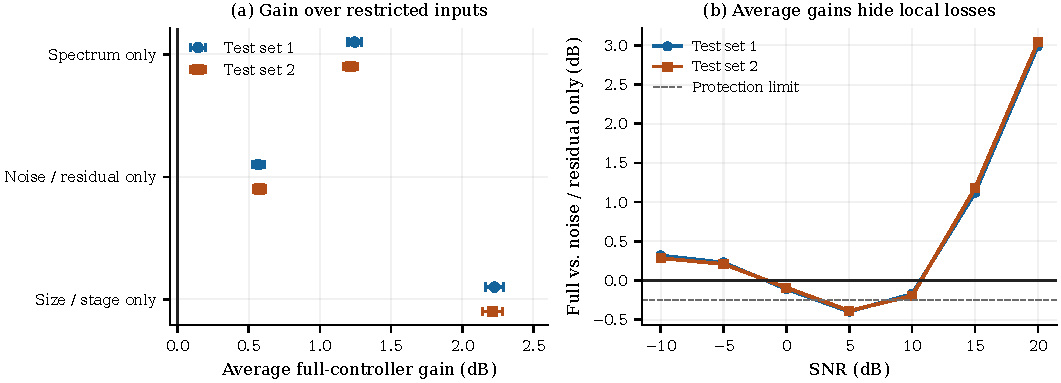
\includegraphics[width=\textwidth]{fig5_features.pdf}
\caption{Original smaller-budget input ablation, unchanged. Full inputs help
the average but fail the declared 0.25~dB protection condition. These are
separate models trained with 4,096 cases, 12 epochs and three seeds; they
are not replacements for the main 16,384-case models.}
\end{figure*}

\subsection{Original Follow-up Comparisons}
The earlier follow-up trains 15 models and evaluates two fresh sets,
each with seven SNR settings and two difficult settings of 200 cases.
The six primary comparisons adjust for multiple testing within each set.
The two new-data adaptive runs use independently generated training data,
one fixed training seed per dataset. They are distinct from the three
main seeds sharing one dataset and from the new reviewer diagnostics.

\begin{table}[!t]
\caption{Original follow-up average gains in dB, unchanged}
\centering\small
\begin{tabular}{@{}p{.68\columnwidth}rr@{}}\toprule
Comparison & Set 1 & Set 2\\\midrule
New-data adaptive vs. global & 2.252 & 2.185\\
New-data adaptive vs. no filtering & 4.250 & 4.191\\
New-data adaptive vs. HS-GS & 1.939 & 1.837\\
Original adaptive vs. supervised & 1.015 & 1.012\\
Original adaptive vs. final-only & 0.697 & 0.694\\
Fixed-open mix vs. original adaptive & 0.064 & 0.066\\\bottomrule
\end{tabular}
\end{table}
The supervised recipe holds architecture, input pilots and training
budget fixed but trains on channel targets with mean linear NMSE.
Selecting its checkpoint by withheld likelihood reduces the gap to
approximately 0.73~dB; pooling linear errors across SNRs reduces it to
about 0.36~dB. It wins in some cases, including two paths. Its transfer
from 21 to 30 pilots was less consistent in validation replay. This
comparison does not establish a general benefit of withholding labels.
The final-only comparison retrains that alternative and its separate
timing sample gives 4.65 versus 2.05~ms; those values do not replace the
main timing table. Fixing mixing at one retains all 188 stored parameters
and worsens two of three seeds on two-path cases, despite its small
average gain.

\section{Historical: Additional Reviewer Diagnostics}
\input{review_diagnostics.tex}

\input{round2_results.tex}

\input{round2_training.tex}

\section{Historical: Related Structural and Sparse Methods}
OptShrink estimates singular-value weights from the observed noise
spectrum~\cite{nadakuditi2014}. LRHD combines that principle with
repeated Hankel projection~\cite{yin2021}; neither our first one-pass
diagnostic nor the new EM/OptShrink adaptation reproduces full LRHD. In both
cases the starting problem is noisy matrix denoising, not recovery from
affine magnitudes. The noise on a Hankel matrix formed from an iterated
channel estimate need not meet asymptotic independent-entry assumptions.
Neither those guarantees nor universal optimality are asserted here.

Structured alternating least squares reconstructs low-rank matrices from
linear measurements, including Hankel structure~\cite{zachariah2012}.
HSGD addresses partially observed Hankel matrices with sparse gross
corruptions~\cite{cai2023}. Their losses, observations and guarantees
cannot be transferred unchanged to our nonlinear Rician model. They
remain important alternative constructions, not irrelevant methods.

Noncoherent compressive channel estimation combines phase retrieval and
sparse reconstruction using a designed sensing cascade~\cite{rasekh2018}.
GP-bandit beam training uses adaptive near-field beams, Rician-debiased
pseudo-amplitudes and sparse phase retrieval~\cite{wang2026}; it has no
known additive reference. Partially coherent matching pursuit retains
complex observations with a shared unknown phase within each
packet~\cite{yi2024}. That information is absent from our magnitude-only
inputs. A fair benchmark must adapt these methods to the same observation
and pilot budget rather than importing their published scores.

The multi-shot Rydberg study~\cite{atapattu2026} concerns signal-presence
detection with Rician shots. It motivates accounting for observation
statistics and shot budgets, but supplies neither channel-estimation
results nor a heavy-tailed noise model for this experiment.

\section{Historical: What Is Still Not Tested}
\textit{Depth.} The new 5/10/20-stage comparison uses separately trained
models, unlike the original prefix diagnostic. It has a fixed small
training budget, not an exhaustive search or a convergence test. An
optimal depth for larger datasets or other channel populations is not known.

\textit{Noise and hardware.} The original model has independent complex
Gaussian noise before magnitude extraction. Incorrect variance inputs
do not test non-Gaussian noise. Finite shot count alone does not imply
heavy-tailed noise, and no cited detection model establishes that
assumption for this receiver. Optical readout, atomic dynamics and
hardware data remain untested. A Rician loss is not automatically matched
to an alternative optical or multi-shot measurement statistic.

\textit{Structure.} Cubic shrinkage is one design choice, not a proved
optimal denoiser. The new in-loop comparison covers one OptShrink-based
reconstruction. Full LRHD, structured ALS and robust Hankel completion
would require their own adapted measurement models and independently
selected settings. Existing hard,
global, adaptive and no-filtering controls do not exhaust these choices.
An angle-domain sparse phase-retrieval method was also missing from this
historical comparison, particularly for two-path channels; the current
compact sparse/EM comparison addresses that gap. No superiority over the
remaining untested methods, or over published URformer, is claimed.

\textit{Training.} Two-path and RSR 5~dB cases already occur in the original
training; RSR 0~dB does not. The new smaller study includes RSR 0~dB,
and its curriculum has mixed results. No safety-critical protection
guarantee follows from average gains. The original pointwise
intervals condition on fixed models and shared training data; the
fresh-data follow-up is limited and does not estimate broad
training-population uncertainty.

\textit{Array geometry.} A two-dimensional array may suggest multilevel
or block-Hankel structure, but its lifting dimensions, normalization,
computational cost and training transfer must be defined anew. No 2D
array result is reported.

\section{Historical: Initialization and Numerical Record}
For array element $n$, form $C_n\in\mathbb C^{P\times(K+1)}$ with rows
$[s_p^T,b_{np}]$. Let $u_n$ be the dominant eigenvector of
$C_n^H\diag(z_n)C_n$ and set
\begin{equation}
 c_n=\frac{\sum_p z_{np}|(C_nu_n)_p|}{\sum_p|(C_nu_n)_p|^2}.
\end{equation}
The first $K$ components of $c_nu_n\exp[-j\arg(u_{n,K+1})]$ initialize
the channel row. In the original training recipe, only the 21 input pilots
enter this calculation; withheld columns do not enter the initial estimate.
The all-pilot alternative instead initializes from its 30-column noisy input view.

The original 43 focused tests cover likelihood and derivative checks,
noise scaling, finite gradients, repeated singular values, pilot-split
isolation, single/double precision agreement and deterministic recovery.
The submission audit recalculated 1,120 main, 702 follow-up and 432
input-study result files. Three primary checkpoints replayed eight saved
observations exactly; 24 input-study checkpoint replays were also checked.
This is not a replay of every historical experiment or an independent
hardware validation.

One finite-input SVD failure occurred in the original classical HS-GS
test at $N=64$. The same matrix was recomputed with SciPy's alternative
SVD driver; relative reconstruction error was below $3\times10^{-15}$.
The trial was retained with unchanged inputs and iteration budget.
Original software versions were Python 3.12, NumPy 2.4.6, SciPy 1.17.1
and PyTorch 2.13.0. The saved local experimental record includes inputs, truth
for evaluation, predictions, selected/final checkpoints, training histories,
settings, source hashes and figure scripts for the reported studies.
The separate Overleaf archive contains manuscript files, not experimental
data. No GPU agreement or hardware measurement is claimed.
\bibliographystyle{IEEEtran}
\bibliography{support/references}
\end{document}
